\documentclass[titlepage]{article}
\usepackage[T1]{fontenc}
\usepackage[utf8]{inputenc}
\usepackage{biblatex}
\usepackage{titling, lipsum}
\usepackage{graphicx}
\usepackage{indentfirst}
\usepackage{geometry}
\usepackage{hyperref} 
\usepackage{float}
\usepackage{enumitem}
\usepackage{array}
\usepackage{booktabs}
\usepackage{longtable}
\usepackage{gensymb}
\usepackage{subfig}

\newcommand{\tabitem}{~~\llap{\textbullet}~~}

\graphicspath{{./images/}{./plots/}}

\geometry{
 a4paper,
 total={170mm,257mm},
 margin=1in
}

\addbibresource{bibliography.bib}

\begin{document}
\begin{titlepage}
	{\centering
	{\scshape\huge Comparison of SLAM methods with CUDA implementation \par}
	\vspace{1cm}
	{\scshape\Large Course: Research project - GPU algorithms \par}}
	
	\vspace{1cm}
	\noindent\textbf{Coordinator}: Kaczmarski Krzysztof\\
	\textbf{Authors}: Rogala Michał, Stasiak Szymon, Śliwakowski Mateusz\\
	\textbf{Description}: This document covers three different SLAM methods with an emphasis on CUDA \mbox{implementation}\\
	\textbf{Code repository}: \href{https://github.com/Sliwson/cuda-slam}{https://github.com/Sliwson/cuda-slam}\\
	\textbf{Code license}: MIT\\
	\textbf{Input files}: Point clouds as .obj files\\

	\vfill
	{\large \today \par}
\end{titlepage}

\tableofcontents
\newpage

\section{Report goals}
%What we will know after reading this document?

The report is devoted to a research of SLAM methods using CUDA technology. We want to give a brief introduction what SLAM is and what are its applications. After reading the document you should know three different methods of approaching the problem, their advantages and disadvantages. The cornerstone of the work is answering the question - how well these methods can be converted to GPU architecture and how much will we gain?

\section{Problem statement}
%Description of the problem, motivating example, killer application, etc.

\subsection{Theoretical background}
\label{sec:theory}
\textbf{Simultaneous localization and mapping} (in short SLAM) is the computational problem of constructing or updating a map of an unknown environment while simultaneously keeping track of an agent's location within it \cite{ms-wiki1}. In theory the problem can be simplified to more mathematical definition - given two point sets $P_1 = \{x_1,\dots, x_n\}$ and $P_2=\{y_1, \dots, y_n\}$ find translation $t$ and rotation $R$ that minimizes the mean square error:
$$MSE(R, t) = \frac{1}{N}\sum_{i=1}{N}(x_i - Ry_i - t)^2$$

The reality, unfortunately, is much more complicated. Sizes of point sets might differ, clouds are unordered and noise points can occur.

\subsection{Applications}
The main field of SLAM application is robotics. There are a lot of machines that utilizes this algorithm to keep track of the space in which they are moving. The most popular are autonomous vacuum cleaners such as presented below.

\begin{figure}[H]
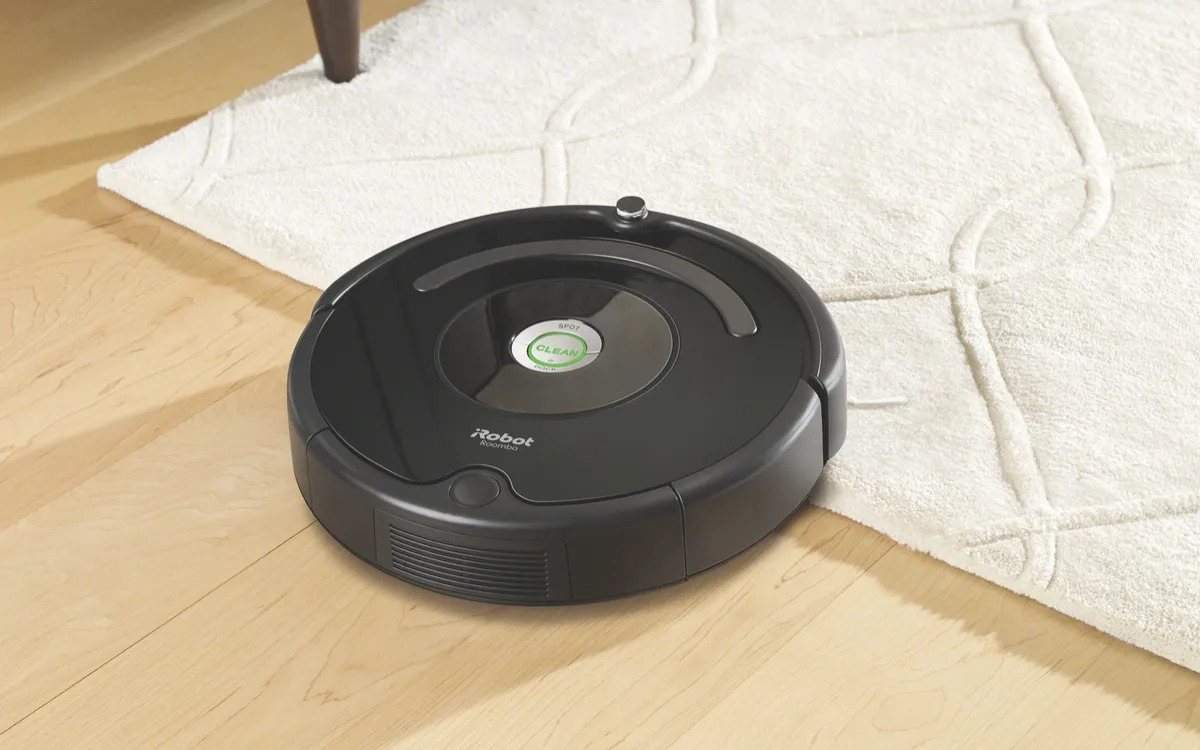
\includegraphics[width=\textwidth]{ms-img1.png}
\caption{Autonomous vacuum cleaner}
\end{figure}

Another popular application is mapping real life environments to digital equivalents. The programs produce \textit{Geospatial mappings} which can be later processed and analysed. Variety of different devices is used such as hand scanners, drone scanners or even satellites. Due to rapid technological progress nowadays, even smartphone cameras can be used to perform simple environmental scan.

\begin{figure}[H]
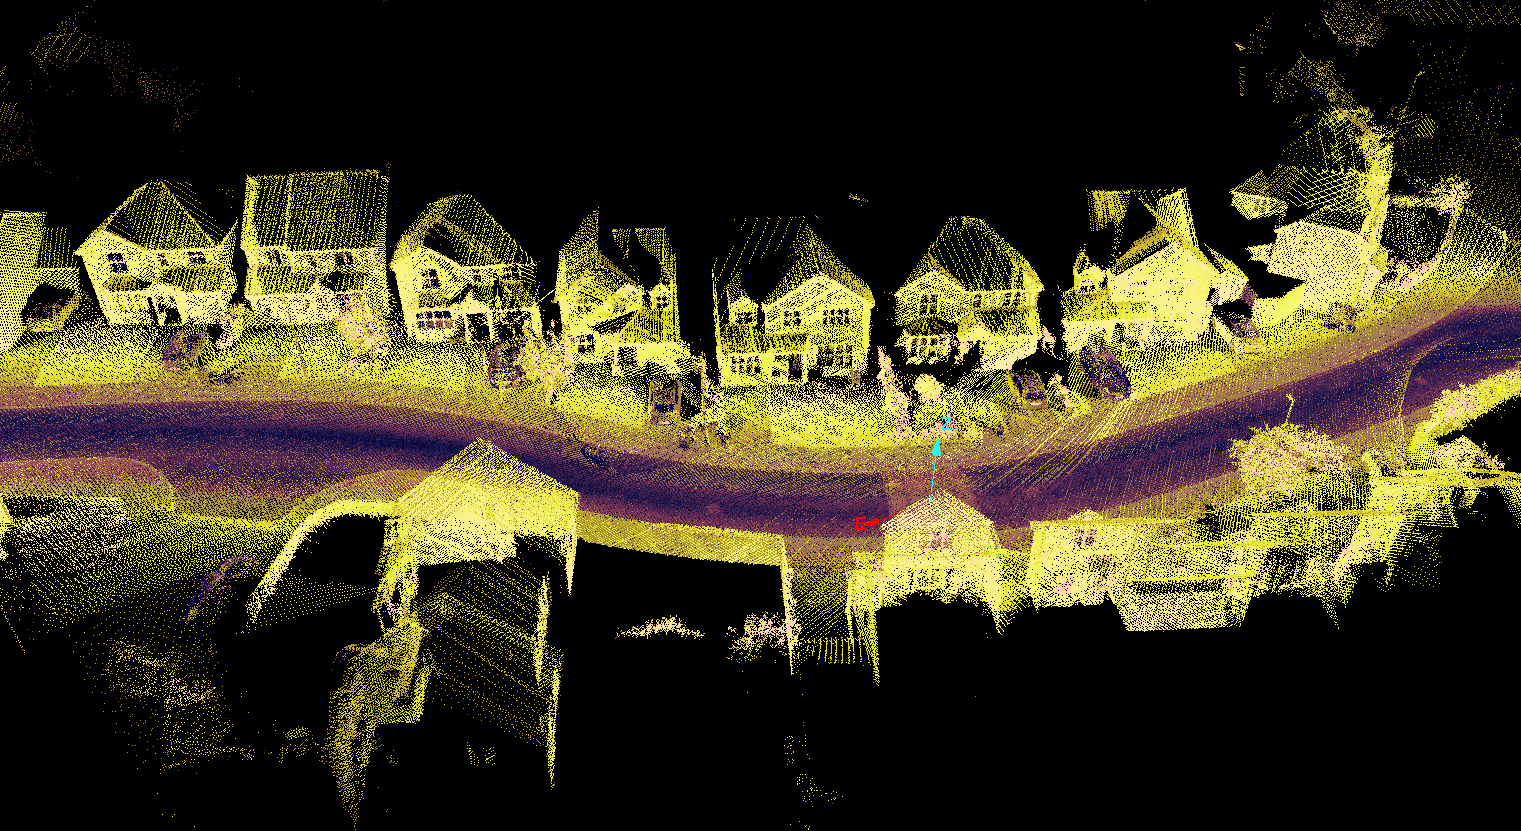
\includegraphics[width=\textwidth]{ms-img2.jpg}
\caption{3D laser scan}
\end{figure}

\section{Computational method}
%The most important ideas in the algorithm necessary to understand how it works.
%Are there any differences from other methods?
%Are there any novel ideas?

\subsection{Iterative Closest Point}
The most widely described and most popular method for solving SLAM problem is Iterative Closest Point algorithm. The main idea of the algorithm is stated below \cite{ms-pres1}:
\begin{enumerate}
\item Determine corresponding points.
\item Calculate translation and rotation using Singular Value Decomposition (in short SVD).
\item Apply calculated rotation and translation to the point cloud.
\item Compute Mean Squared Error.
\item If error decreased and it is greater than given threshold repeat all the steps.
\end{enumerate}

Various modifications have been proposed to this algorithm (such as sampling point sets, weighting the correspondences or rejecting outliers). However, in this project we focused on the base version of the method as it is good enough for comparison with the other algorithms.

\subsection{Non-iterative Closest Point}
Compelling alternative to an iterative point cloud matching algorithms is a non-iterative SVD-based solution. The idea has been described by Shinji Oomori, Takeshi Nishida, and Shuichi Kurogi of Kyushu Institute of Technology. They proclaim that this method is capable of matching clouds even "with less than 4\% of the computational time of the ICP (iterative closest point) algorithm with nearly identical accuracy"\cite{nicp}.\\
The idea of this algorithm can be described in the following points:
\begin{enumerate}
\item Take both point sets (containing respectively $N_1$ and $N_2$ points) and find mass centres for them ($C_1$ and $C_2$).
\item Align the clouds to their mass centres and store the result points in matrices: $A_1$ (size $N_1 \times 3$) and $A_2$ (size $N_2 \times 3$) respectively.
\item Find matrices $U$ from SVD of both matrices, respectively $U_1$ and $U_2$.
\item Rotation matrix is then defined as $R = U_1 \times U_2^T$.
\item Find the translation vector as $t = C_2 - (R \times C_1)$.
\end{enumerate}
Unfortunately, for permuted clouds of different sizes this method does not always converge. That is why one more step is necessary for those conditions:
\begin{enumerate}
\setcounter{enumi}{5}
\item To increase convergence ratio, repeat those steps for multiple scans of observed object and select the transformation minimizing the mean square error (see section \ref{sec:theory}).
\end{enumerate}
This step is indeed a huge improvement but it can be used with promising results only when the item is observed from multiple angles.\\
Implementation described in this paper covers different approach - the copies of source and target clouds are created, each copy with differently permuted points. Transformations received by using steps from 1. to 5. can differ for various permutations, so the result is chosen among them based on the minimal value of mean square error, similarly to what is proposed in the original idea.

\subsection{Coherent Point Drift}

In this method alignment of two point sets is considered as a probability density estimation problem. One point set represents the Gaussian mixture model (GMM) centroids. The second one represents the data points. At the optimum, two point sets become aligned. Method uses Expectation Maximization (EM) algorithm to find scale, rotation matrix and translation vector.\\
Main idea of a coherent point drift algorithm can be presented in several steps:
\begin{itemize}[label={}]
\item E-step:
\begin{enumerate}
\item Compute probabilities matrix P. P describes probability of correspondence of points from both sets.
\end{enumerate}
\item M-step: 
\begin{enumerate}
\setcounter{enumi}{1}
\item Using P and point sets calculate matrix A.
\item Calculate rotation matrix using Singular Value Decomposition of matrix A in a similar way as in the ICP algorithm.
\item Calculate scale and translation vector using point sets and SVD result.
\end{enumerate}
\item Repeat E-step and M-step until convergence.
\end{itemize}
In order not to impair readability we decided to skip mathematical formulas in this schema. Fully detailed description and more information about coherent point drift can be found in article written by Andriy Myronenko and Xubo Song \cite{cpd}.\\
The base version of the algorithm has multiple vulnerabilities, especially when it comes to computation time.
For this reason many improvements are known and some of them have been implemented in our solution. Firstly the size of P matrix is $N \times M$, where $N$ is size of first point set and $M$ is size of second point set. It requires a lot of memory to keep matrix of this size, so instead we can calculate vectors: $P1$, $P^T 1$ and matrix $PX$, where $1$ is vector of all ones and $X$ is first point set. Using these vectors and matrix we can achieve the same result even faster because in calculations we had to multiply P matrix with ones vector and we have already done it.\\
Secondly the main bottleneck of algorithm is the calculation of matrix-vector products $P1$, $P^T1$ and $PX$. This is done with $O(MN)$ complexity. The fast Gauss transform, introduced by Greengard and Strain \cite{fgt}, reduces complexity to only $O(M+N)$.

\section{Program architecture}
%Short description on the modules of the system, requirements, dependencies, etc.
\subsection{Project structure}
The solution consists of three projects:
\begin{itemize}
\item \textit{common} - static library project, contains all elements that are shared between cpu and gpu implementations.
\item \textit{cpu-slam} - executable project, contains implementation of slam methods for cpu and cpu main.
\item \textit{gpu-slam} - executable project, contains implementation of slam methods for gpu and gpu main.
\end{itemize}

\subsection{Modules}
The project is constructed using several modules:
\begin{itemize}
\item \textit{Renderer} - implemented in \textit{common} project. Capable of rendering point clouds in different colors. Can be used multiple times in one executable launch. Widely using for results visualisation.
\item \textit{CloudLoader} - implemented in \textit{common} project. Module responsible for loading .obj point clouds.
\item \textit{Configuration} - implemented in \textit{common} project. Module representing configuration, tightly coupled with \textit{ConfigParser} which allows loading configuration from .json files.
\item \textit{TestRunner} - implemented in \textit{common} project. Module used to define and run benchmarks.
\item \textit{Algorithms} - implemented in \textit{cuda-slam} as well as \textit{cpu-slam}. Each algorithm is implemented in separate file as a global function in appropriate namespace. Some operations that are common for cpu as well as gpu are implemented in \textit{common} project.
\end{itemize}

\subsection{Dependencies}
\begin{itemize}
\item \textit{Assimp} - for cloud loading.
\item \textit{Eigen} - for cpu matrix operations.
\item \textit{Glad} - wrapper for OpenGL.
\item \textit{GLFW} - for window system.
\item \textit{Nlohmann/json} - for configuration parsing.
\item \textit{cuBLAS}, \textit{cuSOLVER} - for gpu matrix operations.
\end{itemize}

\section{Implementation details}
\label{sec:ImplementationDetails}
%What do we thing is worth mentioning when it comes to implementation?
%What path has been chosen to parallelize execution especially for GPU?
%What obstacles have we met when implementing?
%Why have we chosen to use that libraries
\subsection{Common elements}
All of the methods implemented in the scope of this project base to a greater or lesser extent on matrix operations, which have significant impact on computation times and quality of the results. The most important operation is a singular value decomposition (SVD). Apart from that, also large number of less complicated operations, for instance multiplication or addition, are needed. Unfortunately, there is no solid library offering all those functionalities both for CPU and GPU accelerated computations at the same time. For this reason we decided to choose three libraries allowing to receive satisfying results no matter what method is used:
\begin{itemize}
\item \textit{Eigen} - widely recommended, fast and open source library for CPU matrix operations
\item \textit{cuBLAS} and \textit{cuSOLVER} - library created and natively supported by Nvidia for GPU accelerated matrix operations using CUDA technology
\item \textit{glm} - OpenGL Mathematics library used mainly for storing common parts like point clouds, vectors, transformation matrices and basic operations on them. This library is available also for both host and device managed code what allows to reuse some parts of it for CPU and GPU computations and at the same time simplifies visualising the results
\end{itemize}
It is worth clarifying that Eigen has implemented the partial support for CUDA kernels but this feature is still experimental and there are multiple known issues (for example with support for gcc or MS Visual Studio). Adding that to potential problems with performance, we decided not to use this library for GPU accelerated operations in order to maintain higher scalability and stability of the project.

\subsection{Iterative Closest Point}
Because of the fact that for our research we have chosen the simplest method of finding corresponding points across the point sets, the algorithm benefits greatly from using GPU accelerated computations. Each GPU thread is associated with one point from the first cloud and finds the nearest one from the second cloud. It results in almost $100\%$ GPU occupancy and major improvement over CPU computations. Furthermore we used cuSOLVER Singular Value Decomposition although it does not offer as big performance leap as correspondences step.  

\subsection{Non-iterative closest point}
The non-iterative algorithm does not offer too many ways to benefit from parallel CUDA operations. For that reason the most natural path for parallelizing the code is to run SVDs for multiple permutations of source and target clouds on parallel. Unfortunately, natively supported solution from cuSOLVER library - so called "batched SVD" is not an option due to limitations for decomposed matrices size (it cannot be greater than 32 x 32 which corresponds point clouds of 32 points). For that reason another solution has been developed - matrices are decomposed by separate threads in batches of configured size. Implementing this solution also brought multiple issues and the following attempts to obtain expected results can be broken down into several stages:
\begin{enumerate}
\item Running SVD from separate CPU threads - although the SVD methods from cuSOLVER are marked "thread-safe", running them in parallel as CPU threads leaded to memory access violation and program randomly crashed every few times.
\item Running SVD from one CPU thread with separate CUDA streams used for each decomposition - by using this method problems with memory access have been solved, but profiling the application showed that streams run sequentially which is not the result expected.
\item Using separate CPU threads for running decompositions using separate CUDA streams - this method combined the advantages of both approaches, giving truly parallel execution of device managed code, at the same time providing higher parallelization level due to limiting the number of concurrent operations by number of GPU streams instead of CPU threads.
\end{enumerate}

Apart from parallel and sequential variants of Non-iterative Closes Point algorithm, also three different approximation types have been implemented for this method:
\begin{enumerate}
\item \textbf{Full} - to avoid finding corresponding points in each algorithm run, this approximation type bases the error calculation on distance between two points with the same indexes in both clouds. It offers promising results with fast calculations for insufficiently permuted clouds but otherwise the error approximation might differ from actual one and for this reason returned result might not be the best.
\item \textbf{None} - after each repetition, error is calculated by finding correspondences between subcloud of given size taken from first cloud and the entire second cloud. This method offers higher reliability but instead increases the execution time of one iteration noticeably, especially using CPU.
\item \textbf{Hybrid} - error for each run is calculated the same way as using when using full approximation but 5 best results are stored and the error is recalculated for those in the same as when using none as approximation type (with finding correspondences). Then, the one with the smallest error is returned as an actual result.
\end{enumerate}

\subsection{Coherent point drift}

CPU solution of coherent point drift is based on algorithm description described in \cite{cpd}. It also uses Matlab code provided by authors as an example how some technical details were handled. FGT algorithm implementation is based on Matlab implementation available here \cite{fgtmatlab}.
Parallelized solution using GPU acceleration mainly focuses on matrices multiplication using cuBLAS and using thrust whenever possible. FGT algorithm was not implemented on GPU due to complexity of this solution and lack of reliable external implementation.

Three different approximation types have been implemented for this method:
\begin{enumerate}
\item \textbf{None} - Probabilities are calculated without FGT.
\item \textbf{Full} - Uses only FGT to calculate probabilities.
\item \textbf{Hybrid} - FGT is used only when error is above certain level.
\end{enumerate}

\subsubsection{Parameters}

\section{Input data description}
%File formats, api used to read, dependencies, data sources, etc.
%Is there any institution providing the input data?
%References to public databases.

As we wanted to keep the input simple we decided to use .obj files as the point clouds. It is easy to find multiple different models in this format which allowed us to test the algorithms on multiple distinctive samples. Furthermore, one can edit .obj files using for example \textit{Blender} to add noise or even cut off part of the cloud. We found that method most convenient to simulate real life conditions as 3D scanners data has to be processed using methods that are beyond the scope of our work.

\begin{figure}[H]
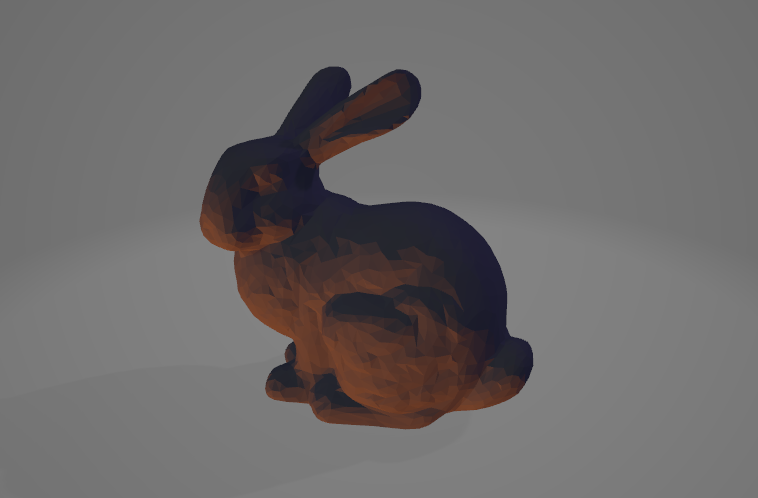
\includegraphics[width=\textwidth]{ms-bunny.png}
\caption{Sample .obj file}
\end{figure}

\section{Execution, configuration and user guide}
%How can one replicate the experiments?
%Any relevant information and runtime howtos.
\subsection{Execution}
Currently the only supported operating system is Windows and the Visual Studio environment as a development tool. All the requested libraries are included in the solution folder and the application should be able to run out of the box on supported environments with Cuda Toolkit 10.2 and common C++ libraries. Necessary configuration files and schemas for config files are attached as well. Each executable (for both CPU and GPU implementations) are supposed to handle 0 or 1 command line parameters with following results:
\begin{itemize}
\item No parameters - load config from default.json
\item One parameter (config file name) - load config from given file
\begin{figure}[H]
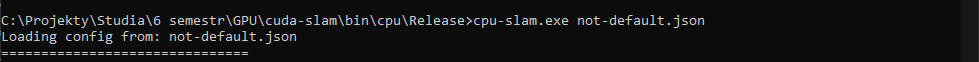
\includegraphics[width=\textwidth]{ss-exec.png}
\caption{Execution example with given config file}
\end{figure}
\end{itemize} 

Support for Linux systems and other development tools are some of the areas of improvement for the future. Porting, however, is not supposed to be an issue. But due to multiple dependencies between used libraries we decided not to focus on it in development phase as it is not the point of this research.

\subsection{Configuration}
Possible fields and values for config files are defined by \textit{JSON Schema} and they are described in the table below.

\begin{center}
\def\arraystretch{1.5}
\begin{longtable}{ | m{13em} | m{5em} | m{3em}| m{19em}| } 
 \hline
 Field name & Type & Default Value & Description \\
 \hline
 \hline
 *before-path & String & -- & Path to the first point set (also called "cloud before") representing object before transformation. \\
 \hline
 *after-path & String & -- & Path to the second point set (also called "cloud after") representing object after transformation. This cloud is to be modified by applying scale, transformation and rotation values mentioned below. \\
 \hline
  & & & Selected algorithm. Possible values are: \\
  *method & Enum & -- & \tabitem icp - Iterative Closest Point \\
  & & & \tabitem nicp - Non-iterative Closest Point \\
  & & & \tabitem cpd - Coherent Point Drift \\
 \hline
  & & & Use sequential or parallel computations on CPU. Possible values are:\\
 policy & Enum & parallel & \tabitem sequential \\
  & & & \tabitem parallel \\
  & & & Used only for ICP and NICP. \\ 
 \hline
 scale & Number & $1.0$ & Transformation scale. Scales the second point set by given value. \\ 
 \hline
 translation & Array: Length $3$ & -- & Translation vector. Translates the second point set by given value. \\ 
 \hline
 rotation & Array: Length $9$ & -- & Rotation matrix in row-major order. Represents the rotation which is to be applied to the second point set. \\ 
 \hline
 translation-range & Number & -- & Translation distance to be applied to the second point set. Translation direction is chosen randomly. \\ 
 \hline
 angle-range & Number & -- & Translation angle in radians to be applied to the second point set. Rotation axis is chosen randomly. \\ 
 \hline
 max-iterations & Integer & -- & Maximum number of iterations for iterative algorithms - ICP and CPD. After reaching this value, algorithm stops returning the best match found so far. \\ 
 \hline
 cloud-before-resize & Integer & -- & Desired number of points in the first point set. If value is given, the set will be resized to this size omitting randomly selected points. Otherwise, whole cloud will be used. \\ 
 \hline
 cloud-after-resize & Integer & -- & Desired number of points in the second point set. If value is given, the set will be resized to this size omitting randomly selected points. Otherwise, whole cloud will be used. \\ 
 \hline
 cloud-spread & Number & -- & The maximum distance in a single dimension between the extreme points in second point set. Based on this value cloud can be stretched or shrunk. \\ 
 \hline
 random-seed & Integer & -- & A seed for random number generator used in the program. If value is not given, the seed is random as well. \\ 
 \hline
 show-visualisation & Boolean & False & Specifies if graphic visualisation of clouds should be displayed. \\ 
 \hline
 max-distance-squared & Number & $1000.0$ & Maximum distance to search for closest point in ICP algorithm implemented on CPU. If the squared distance between two points is larger than value of this parameter, then this pair is excluded from further analysis. \\ 
 \hline
 approximation-type & Enum & hybrid & Approximation variant used for CPD or Non-iterative Closest Point methods. More details about those types are covered in sections devoted to the methods. \\ 
 \hline
 nicp-batch-size & Number & $16$ & Number of Non-iterative Closest Point repetitions run simultaneously. Used only on GPU as the CPU always uses hardware concurrency (number of actual threads in CPU). \\ 
 \hline
 nicp-iterations & Number & $32$ & Total number of repetitions for Non-iterative Closest Point algorithm. \\ 
 \hline
 nicp-subcloud-size & Number & $1000$ & Number of points taken for error computation in Non-iterative Closest Point algorithm \\ 
 \hline 
 cpd-weight & Number & $0.3$ & Weight of the uniform distribution that accounts for noise and outliers in Coherent Point Drift algorithm. \\ 
 \hline
 cpd-const-scale & Boolean & False & Coherent Point Drift parameter, its value indicate if both clouds are assumed to be in the same scale. \\ 
 \hline
 cpd-tolerance & Number & $1e-3$ & Minimum relative error value between subsequent iterations for Coherent Point Drift algorithm, indicating if the algorithm should stop computations as if the match was found. \\ 
 \hline
 convergence-epsilon & Number & $1e-3$ & Minimum error value for indicating if the point sets are treated as matched. Used in all methods. \\ 
 \hline
 noise-affected-points-before & Number & $0.0$ & Ratio (in range $[0.0, 1.0]$) of points from the first point set which should be affected by noise. \\ 
 \hline
 noise-affected-points-after & Number & $0.0$ & Ratio (in range $[0.0, 1.0]$) of points from the second point set which should be affected by noise. \\ 
 \hline
 noise-intensity-before & Number & $0.1$ & Noise intensity for first point set. Noise is then applied by translating each dimension of each point by random value limited by the value of this parameter multiplied by \textit{cloud-spread} value. \\ 
 \hline
 noise-intensity-after & Number & $0.1$ & Noise intensity for second point set. Noise is then applied by translating each dimension of each point by random value limited by the value of this parameter multiplied by \textit{cloud-spread} value. \\ 
 \hline
 additional-outliers-before & Integer & $0$ & Number of randomly generated points added into the first point set. \\ 
 \hline
 additional-outliers-after & Integer & $0$ & Number of randomly generated points added into the second point set. \\ 
 \hline
 fgt-ratio-of-far-field & Number & $10.0$ & Ratio of far field used in Fast Gauss Transform. Applies only to Coherent Point Drift algorithm with hybrid or full approximation. \\ 
 \hline
 fgt-order-of-truncation & Integer & $8$ & Order of truncation used in Fast Gauss Transform. Applies only to Coherent Point Drift algorithm with hybrid or full approximation. \\ 
 \hline
 fgt-ratio-of-far-field & Number & $10.0$ & \\ 
 \hline
 fgt-order-of-truncation & Integer & $8$ & \\ 
 \hline
 \caption{Configuration}
\end{longtable}
\label{tab:configuration}
\end{center}
\textit{* - field is required}

\subsection{GUI}
Both GPU and CPU programs implement the possibility to display visualisation of point clouds using OpenGL. By default, the window display three cloud sizes of different color:
\begin{itemize}
\item Red - the first point set (also called "cloud before")
\item Green - the second point set (also called "cloud after")
\item Yellow - first point cloud transformed with result transformation
\end{itemize}

The visualisation window also supports some basic user control. All the possible actions are described in the table below.
\begin{center}
\def\arraystretch{1.5}
\begin{longtable}{ | m{13em} | m{27em}| } 
 \hline
 Action & Result \\
 \hline
 \hline
 Escape & Close the visualisation. \\
 \hline
 Mouse movement & Rotate the camera. \\
 \hline
 WSAD & Move the camera (front, back, left, right). \\
 \hline
 Spacebar & Move the camera up. \\
 \hline
 Left Shift & Move the camera down. \\
 \hline
 Scroll & Zoom. \\
 \hline
 1 & Toggle visibility of the first point set. \\
 \hline
 2 & Toggle visibility of the second point set. \\
 \hline
 3 & Toggle visibility of the transformed point set. \\
 \hline
 4 & Toggle visibility of the (0,0) point. \\
 \hline
 [ & Reduce the point size. \\
 \hline
 ] & Increase the point size. \\
 \hline
 \caption{Renderer controls}
\end{longtable}
\label{tab:controls}
\end{center}

\section{Description of the results}
%Performance of the system for different input data/parameters.
%How we understand the results and why are they correct?
%Can we formulate any conclusions from the experiments?

\subsection{Execution times}
\subsubsection{Introduction}
We did not expect CUDA implementations to bring better stability or noise tolerance but we did hope to achieve major improvements in terms of the methods execution times. All the performance tests were run on the machine with the following configuration:
\begin{itemize}
\item CPU - AMD Ryzen 7 2700X, 8 cores, 16 threads, 3.7 GHz
\item GPU - NVIDIA GeForce RTX 2060 SUPER
\item RAM - DDR4 16GB, 3333 MHz, CL16
\end{itemize}

Different point clouds were used depending on test size:
\begin{itemize}
\item $0 - 14904$ points - \textit{bunny.obj}
\item $14905 - 35008$ points - \textit{bird.obj}
\item $35009 - 333536$ points - \textit{rose.obj}
\item $333537 - 376401$ points - \textit{mustang.obj}
\item $376402 - 1375028$ points - \textit{airbus.obj}
\end{itemize}

To achieve a reasonable rate of convergence we decided to test the clouds without any noise and outliers. We used transformation with $0.2\: rad$ rotation and translation with magnitude of $10$ units for clouds of size bounded by cube with an edge which length equals $10$ units. It is worth noting that the times presented on the charts contains resource allocation and release.

\subsubsection{Iterative Closest Point}
For Iterative Closest Point method we run benchmarks using one-threaded CPU solution, multi-threaded CPU solution and CUDA-accelerated solution. On the charts a single iteration time is presented because different runs result in different iterations count which makes the results hard to interpret. The results are presented using logarithmic scale as the differences between variants of the algorithm are significant.

\begin{figure}[H]
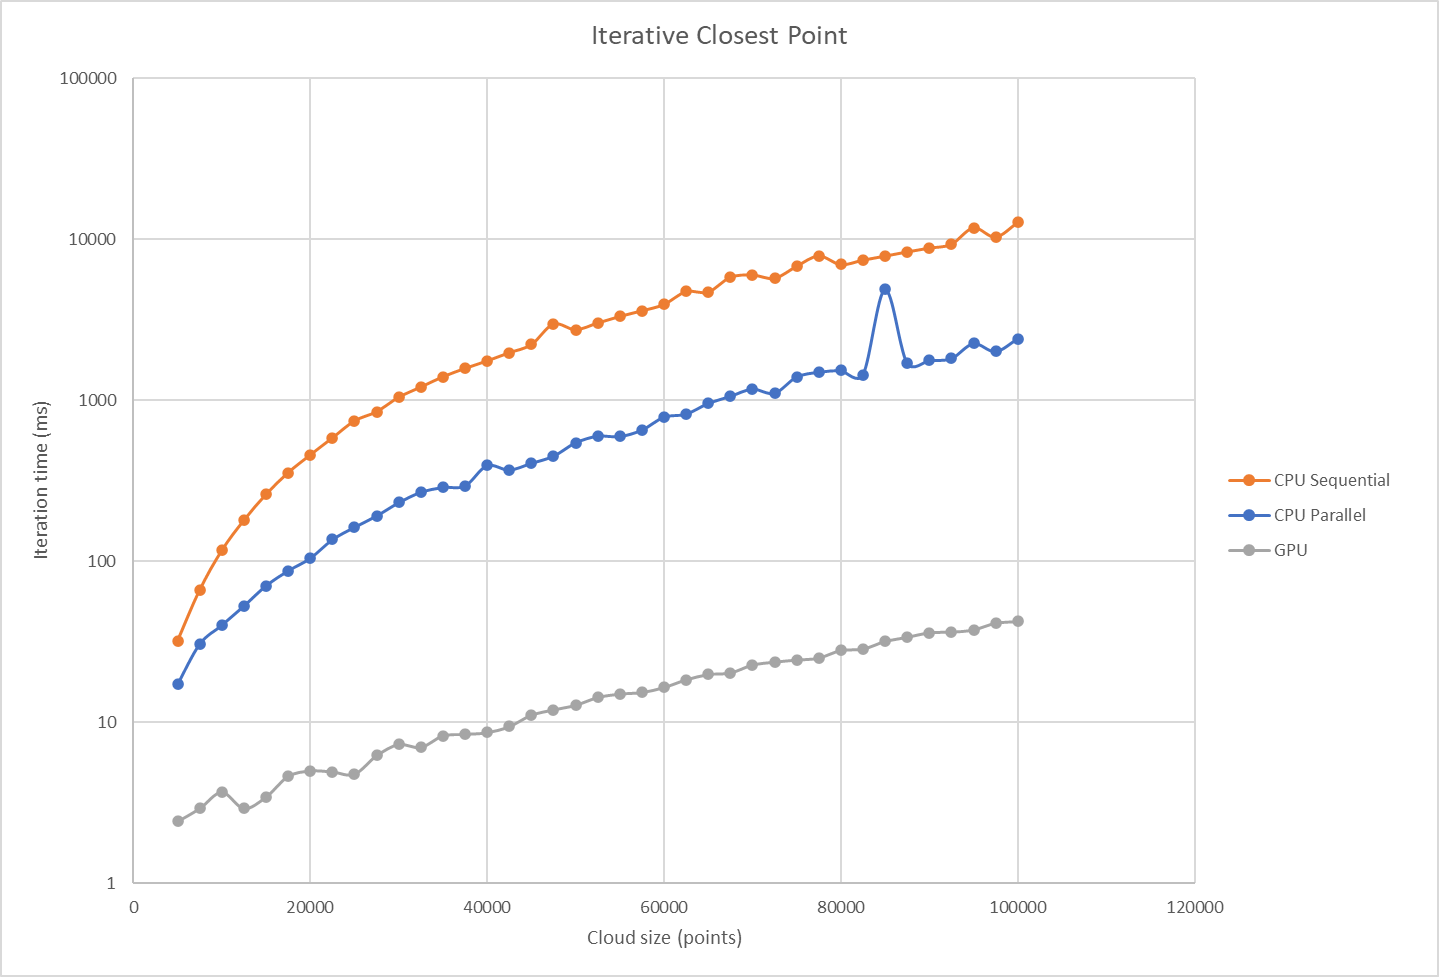
\includegraphics[width=\textwidth]{ms-icp-1.png}
\caption{Results of the benchmark for CPU Parallel, CPU Sequential and GPU implementations of the ICP method}
\end{figure} 

As we can see, the benchmarks prove the expectations and parallelization of the ICP algorithm results in big performance improvements. Having iteration time lower than 100ms for clouds with size of $100000$ points more tests could be run for the GPU implementation.

\begin{figure}[H]
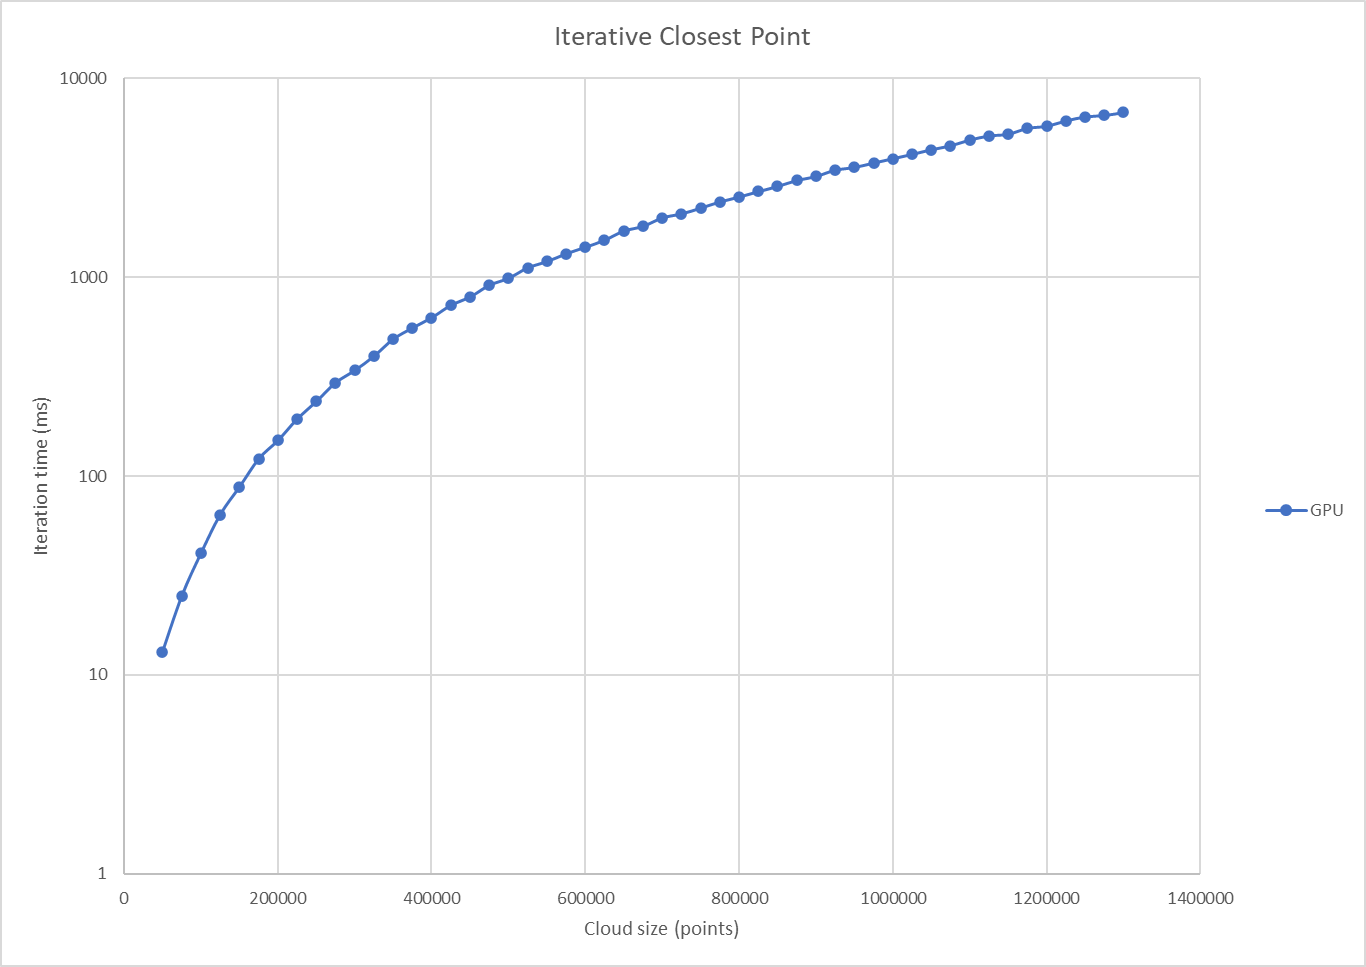
\includegraphics[width=\textwidth]{ms-icp-2.png}
\caption{Results of the benchmark for GPU implementation of the ICP method}
\end{figure}

Even for clouds with size over $1000000$ points one iteration lasts less than 10s which is a reasonable amount. The benchmarks show that the CUDA-accelerated solution is a perfect choice when utilizing the ICP algorithm.

\subsubsection{Non-iterative closest point}
Non-iterative closest point method is performance-wisely a truly interesting one. We expect it to be the fastest because it requires only matrix multiplication and singular matrix decomposition. To avoid an overwhelming amount of information on one chart we split comparisons to separate ones. Because only setting approximation mode to \textit{None} results in a different iteration count in each run we present benchmarks for the whole runs, not single iterations as in ICP section. The maximum iterations parameter is set to $64$, batch size to $16$ and subcloud size to $1000$. We found normal scale on y axis the most suitable to present the results.

\begin{figure}[H]
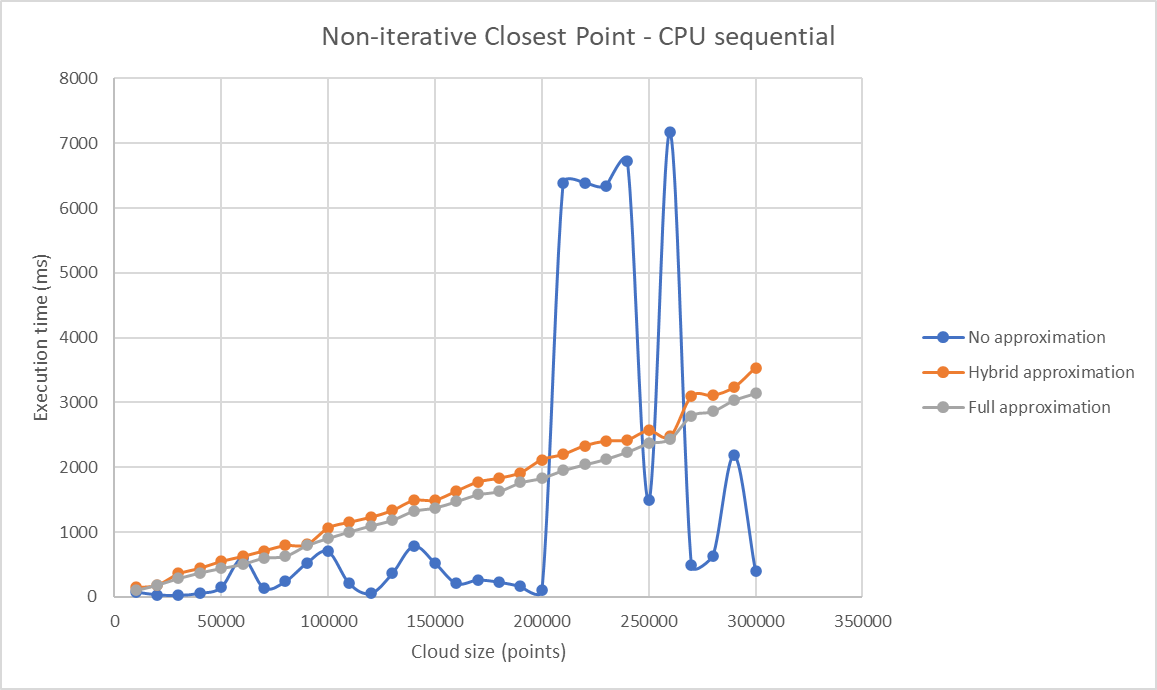
\includegraphics[width=\textwidth]{ms-nicp-1.png}
\caption{Results of the benchmark for sequential CPU implementation of the Non-iterative Closest Point method}
\end{figure}

\begin{figure}[H]
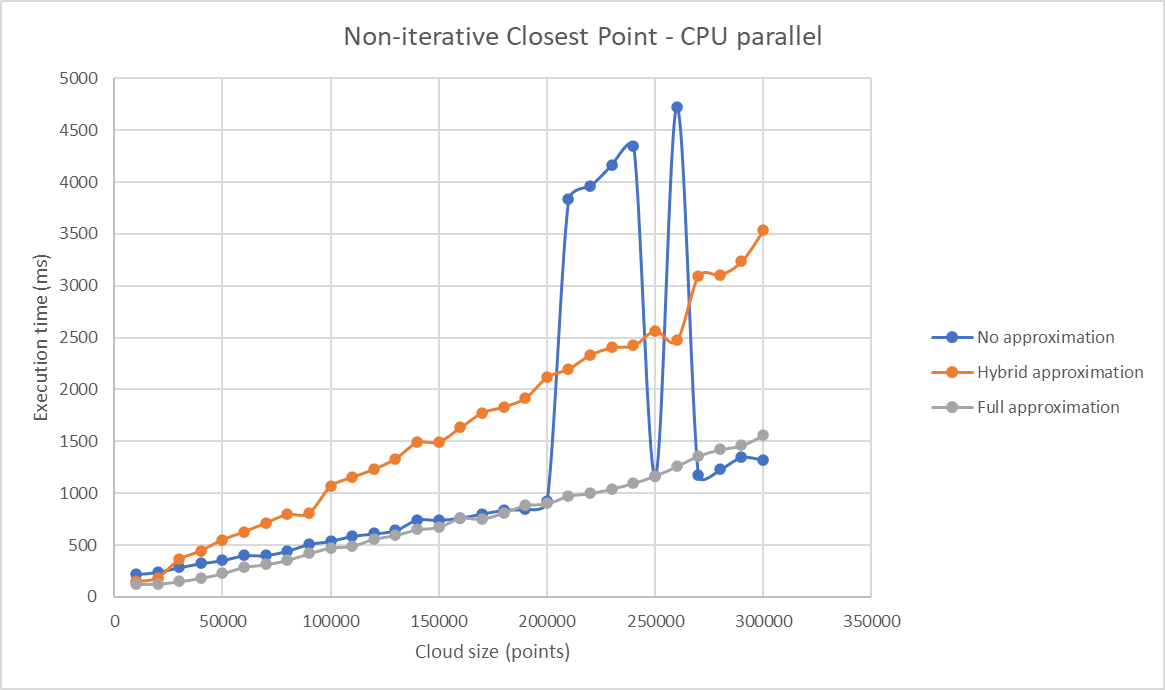
\includegraphics[width=\textwidth]{ms-nicp-2.png}
\caption{Results of the benchmark for parallel CPU implementation of the Non-iterative Closest Point method}
\end{figure}

\begin{figure}[H]
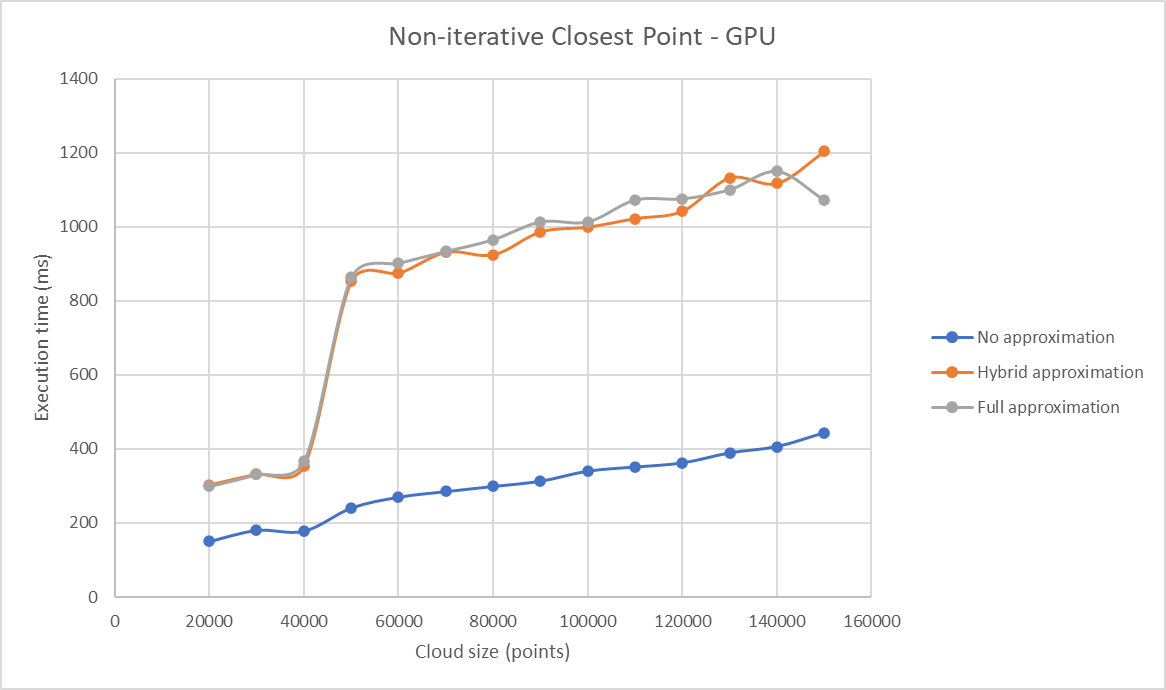
\includegraphics[width=\textwidth]{ms-nicp-3.png}
\caption{Results of the benchmark for GPU implementation of the Non-iterative Closest Point method}
\end{figure}

The benchmarks have clearly shown that in practical usages the version without any approximation yields the best results. We expected \textit{Hybrid} and \textit{Full} approximation to improve overall performance, although the tests have shown that calculating the error each step is a better choice than approximating it and choosing the result after all iterations are finished.

\begin{figure}[H]
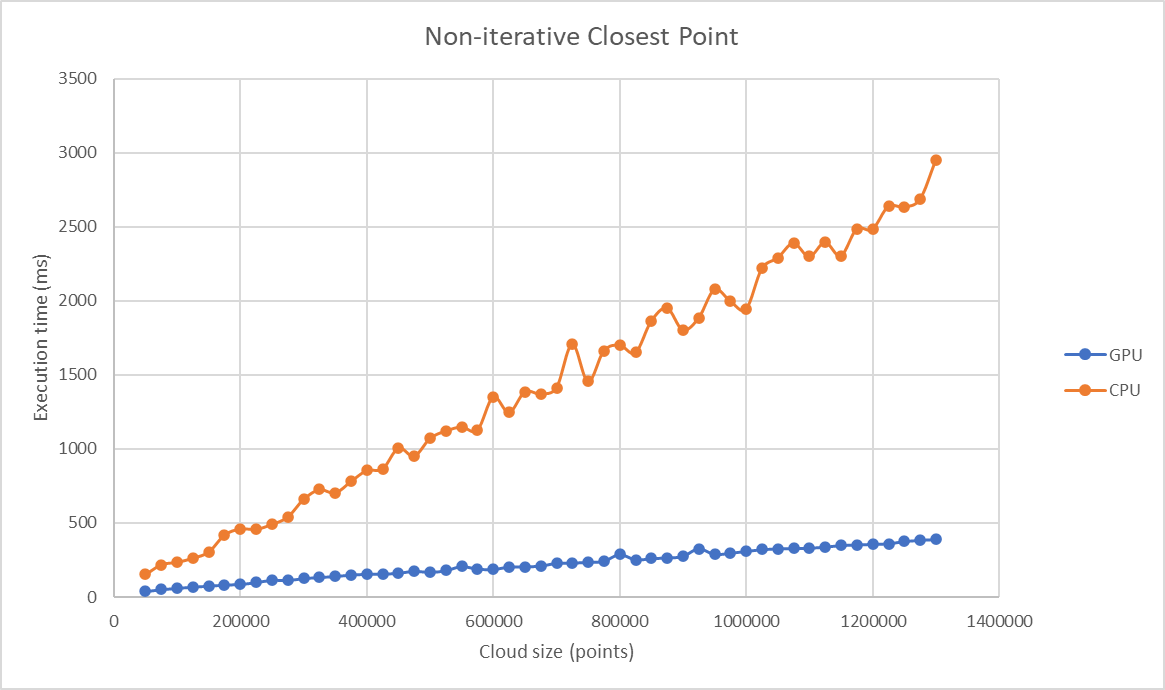
\includegraphics[width=\textwidth]{ms-nicp-4.png}
\caption{Results of the benchmark for CPU and GPU implementation of the Non-iterative Closest Point method}
\end{figure}

To the benchmark comparing the GPU and CPU implementations we chose the most performant variants of the algorithms. The CUDA-accelerated implementation proved to be faster than the CPU parallel. It is worth noting that for cloud over $1000000$ points it achieves execution time below $500\: ms$. 

\subsubsection{Coherent Point Drift}
Coherent Point Drift algorithm was the hardest to implement and it is certainly the most complicated considering the scope of our research. Therefore we do not expect CUDA solution to bring significant improvement in this case.

For the performance tests \textit{weight} parameter was set to $0.1$ and \textit{const-scale} to $false$. The other parameters were the same as in other benchmarks. We present the results using logarithmic scale on y axis. Similarly to Non-iterative Closest Point benchmarks we compare three approximation types, this time approximations relying on using Fast Gauss Transform.

\begin{figure}[H]
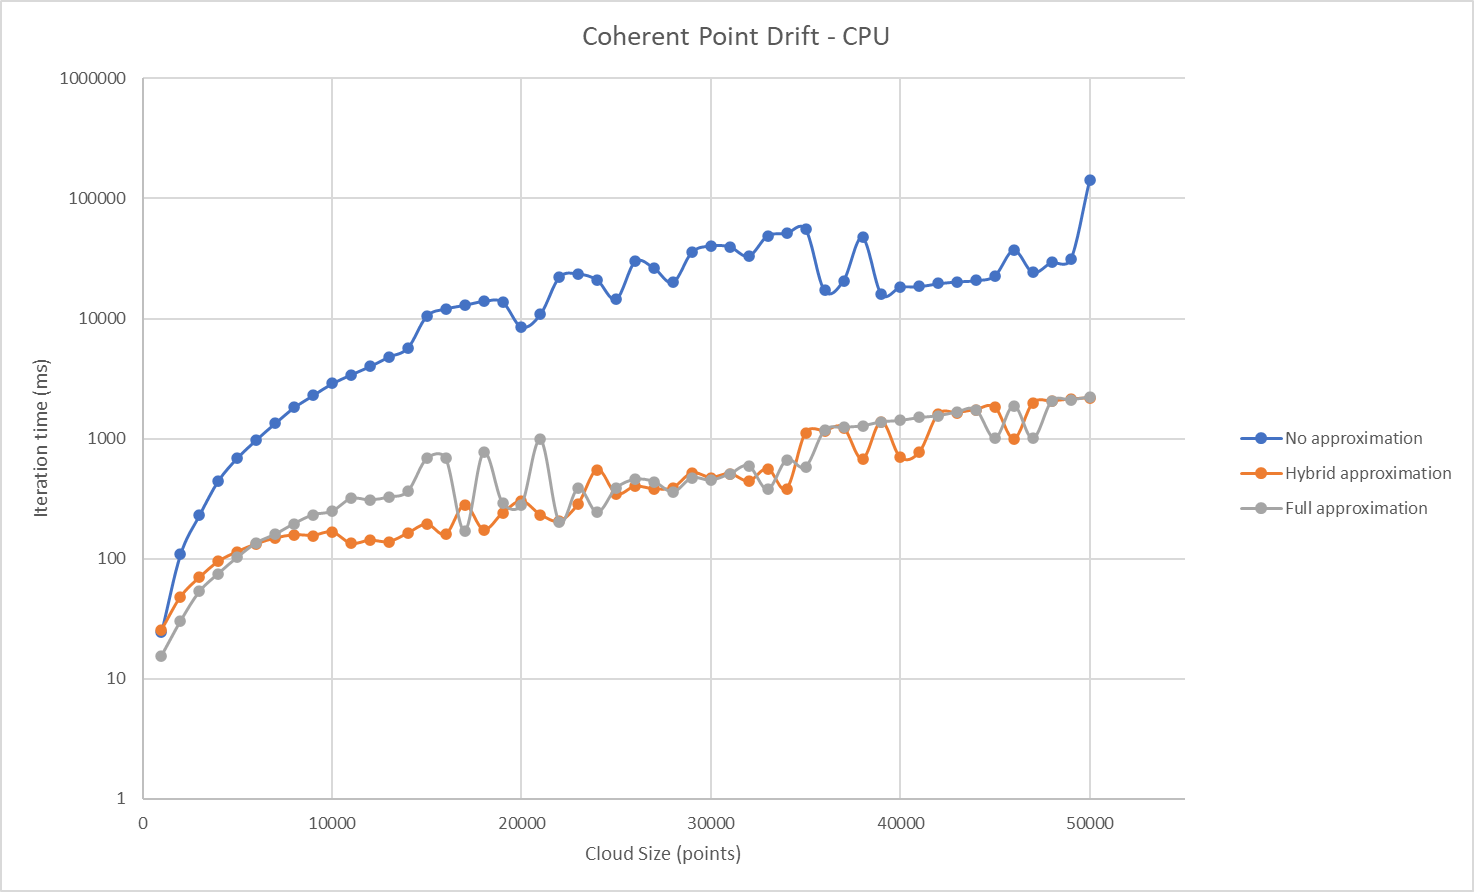
\includegraphics[width=\textwidth]{ms-cpd-1.png}
\caption{Results of the benchmark for CPU implementation of the Coherent Point Drift method}
\end{figure}

\begin{figure}[H]
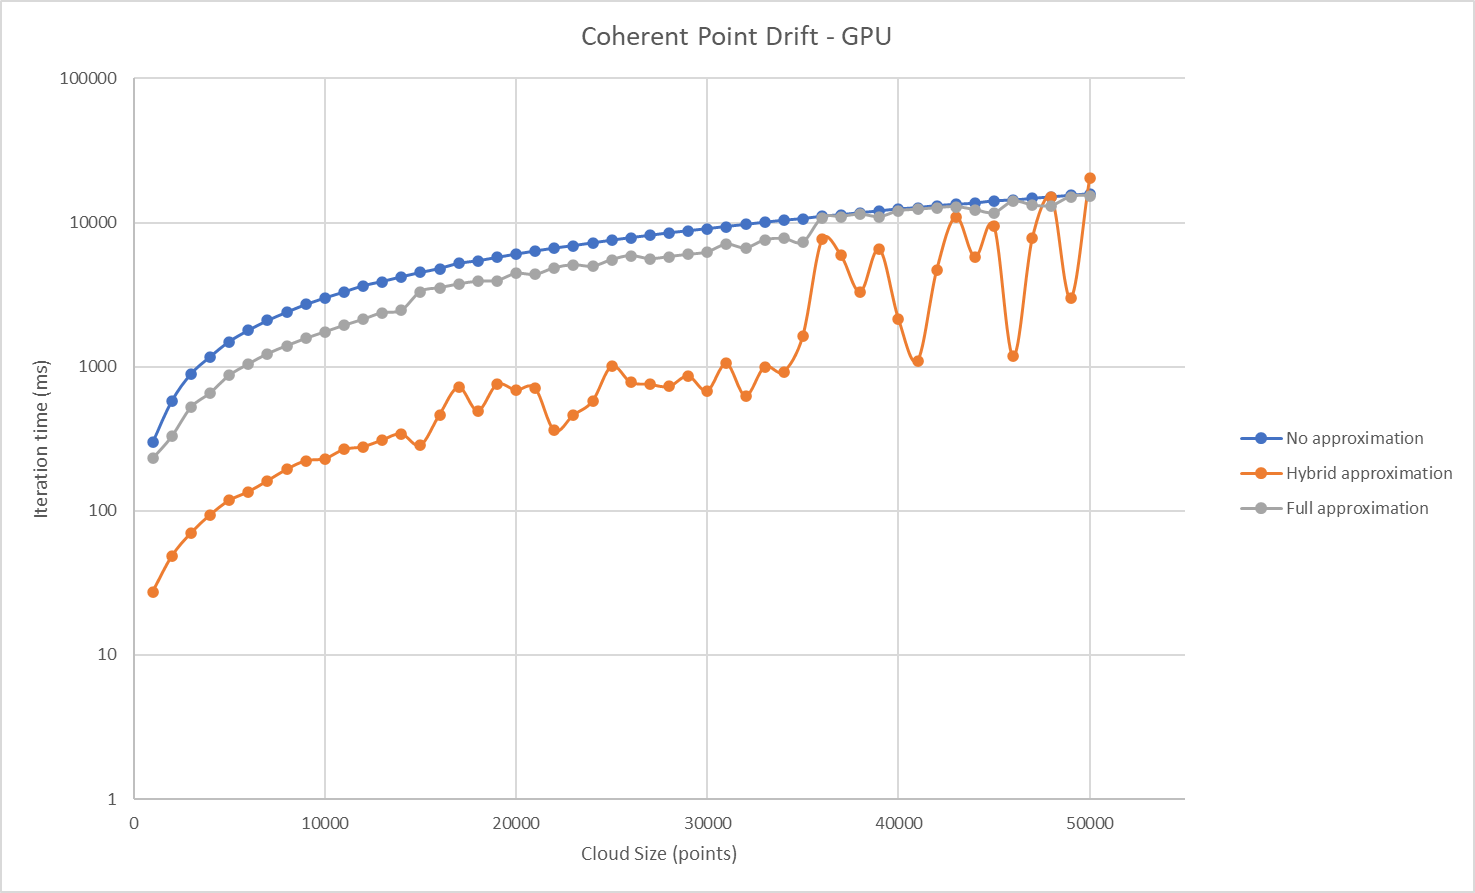
\includegraphics[width=\textwidth]{ms-cpd-2.png}
\caption{Results of the benchmark for GPU implementation of the Coherent Point Drift method}
\end{figure}

\begin{figure}[H]
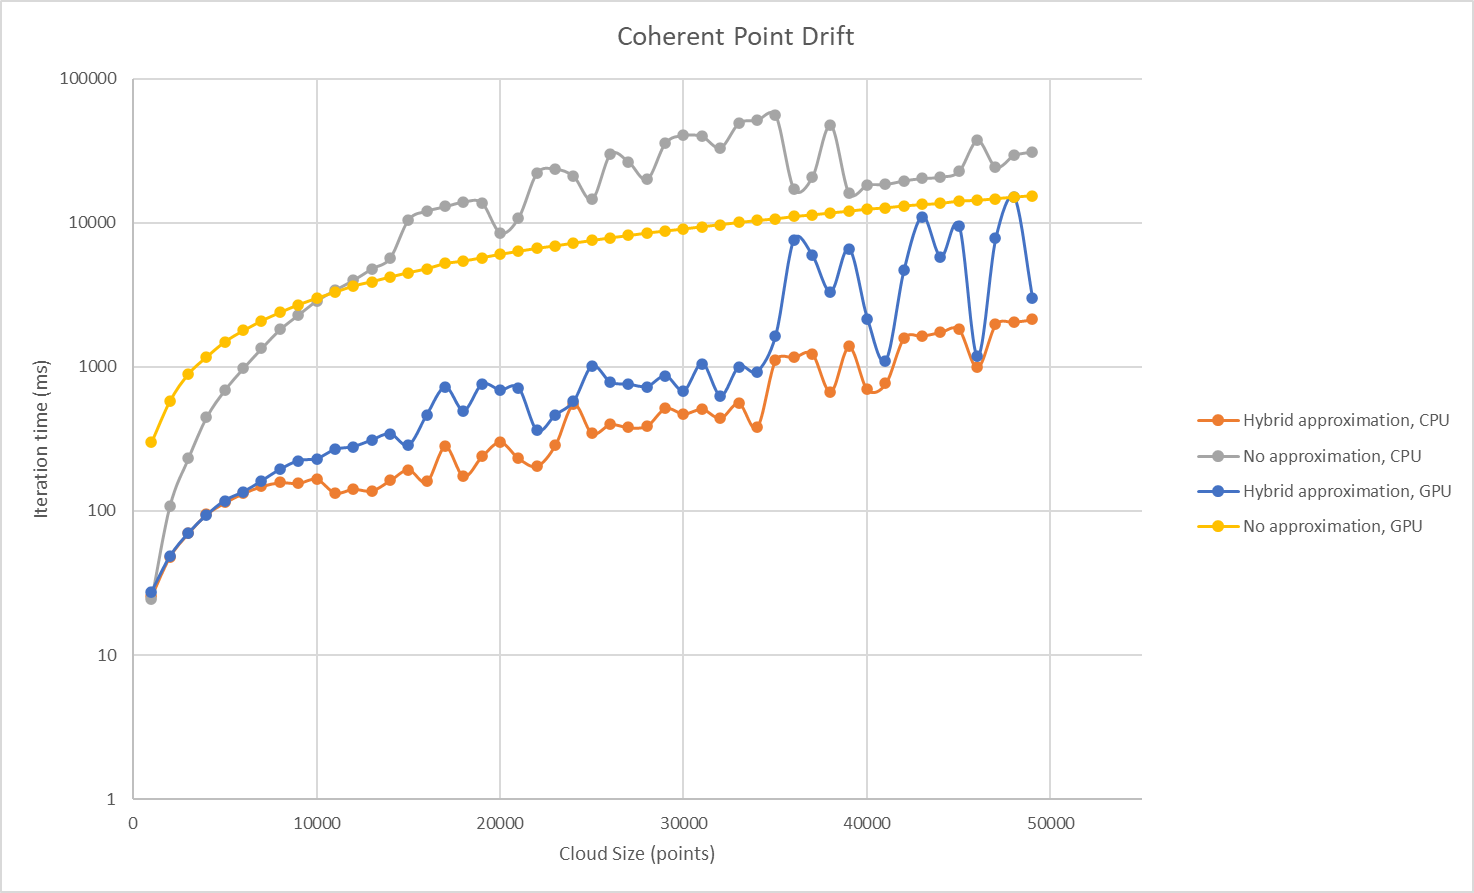
\includegraphics[width=\textwidth]{ms-cpd-3.png}
\caption{Results of the benchmark for CPU and GPU implementation of the Coherent Point Drift method}
\end{figure}

We can note that implementations utilising Fast Gauss Transform are considerably faster than the ones without approximation. GPU acceleration did not bring satisfying improvements, however the variant without approximation is an exception because it is fastest and gives more predictable execution times than CPU implementation.

\subsubsection{Methods comparison}

To sum up the section describing execution times, we gathered all the methods benchmarks on one chart. The parameters were the same as in all the other benchmarks, however this time an execution time is presented for all the methods. Because the differences between all the variants are substantial we used a logarithmic scale on y axis.

\begin{figure}[H]
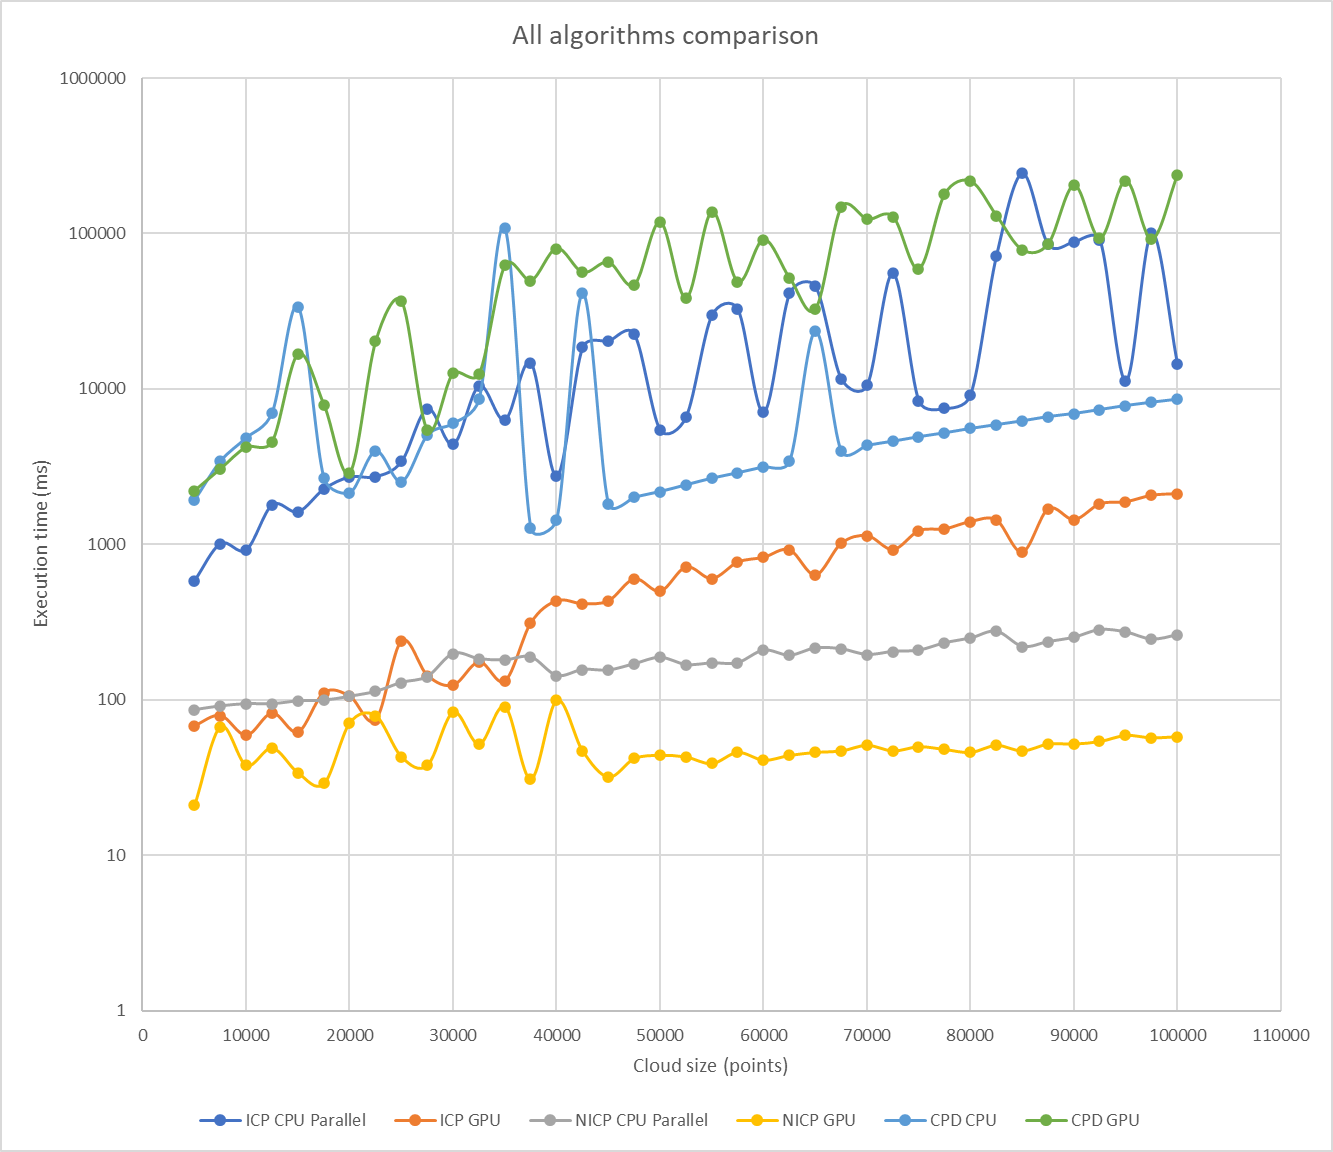
\includegraphics[width=\textwidth]{ms-all.png}
\caption{Comparison of all methods execution times}
\end{figure}

As we can see the execution times differ vastly depending on method and execution policy. We are satisfied with the results especially for Iterative Closest Point and Non-iterative Closest Point methods because we managed to significantly improve the performance by utilizing CUDA library. Therefore, these two methods would be the best choice if time is the most important factor while utilizing SLAM. Coherent Point Drift was expected to be the slowest of the all methods due to its sophistication. However its CPU implementation using Fast Gauss Transform occurred to be faster than ICP CPU variant and it is usable even for clouds with considerable sizes.

\subsection{Noise and outliers tolerance}
We tested our methods using the clouds and conditions that may be closer to reality. That is, we used clouds that are missing points or even entire part and we corrupted clouds by noise and outliers. For this purpose we have used CPU versions of algorithms. For ICP and NICP \textit{policy} was set to \textit{parallel} and \textit{approximation-type} to \textit{none}. For CPD \textit{approximation-type} was set to \textit{hybrid}, mainly to achieve faster computation times. Many tests were conducted and it turned out that results are highly dependent on configuration. Therefore, we will show the most interesting results and tests that have shown the most consistent characteristics.\\
After testing we came to several conclusions. Firstly, the ICP algorithm coped the worst with almost all test sets. The main reason can be cloud sizes used in tests, which occurred to be often too big for ICP capabilities. Algorithm had also trouble with noise. Even low level noise such as $noise-aafected-points-before=0.1$ and $noise-intensity-before=0.05$ may cause convergence failure. Secondly, increasing $max-iterasions$ can help achieving more exact results. CPD algorithm mostly achieved correct results. Main key to CPD convergence is to select parameters value correctly. The most important one is \textit{cpd-weight} which describes how many points 
are noise and outliers. Difference of $0.3$ can lead to significantly different result. Second CPD parameter is \textit{cpd-const-scale}. Setting it to \textit{true} may help achieving better results when we know that the scale did not change after transformation. Especially it helps when clouds contain a lot of noise and outliers. Also, decresing \textit{cpd-tolerance} and \textit{converge-epsilon} (the latter applies also to ICP and NICP) may result in increasing iterations count and lead to more exact result.\\
All algorithms had tendency to match areas where the point density was the highest. An example of this behavior may be observed using \textit{Config21.json} available here: "DEJ LINK DO GITHUBA". It uses two "airbus" clouds with decreased sizes and added noise and outliers. Result achieved by algorithms are presented below and vary among each other.

\begin{figure}[H]
	\centering
    \subfloat[\centering CPD]{{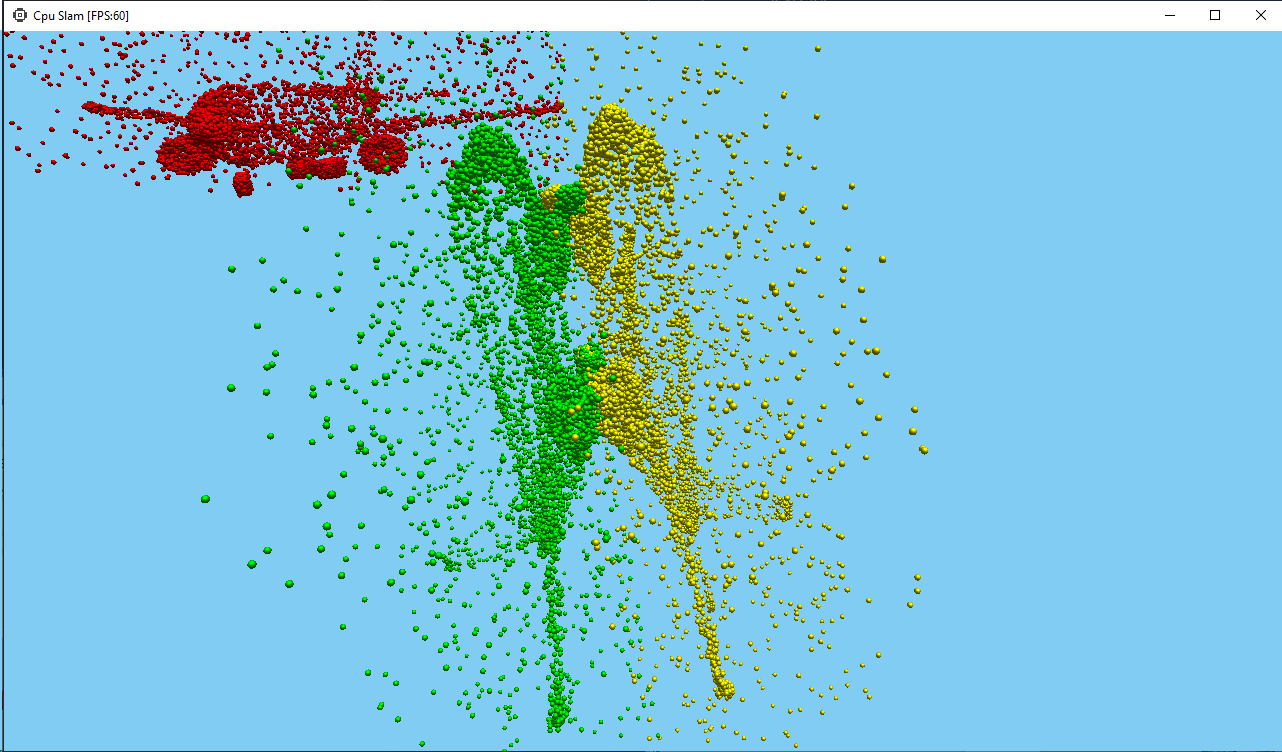
\includegraphics[width=5cm]{mr-cpd-21.png} }}
    \hspace{0.5em}
    \subfloat[\centering ICP]{{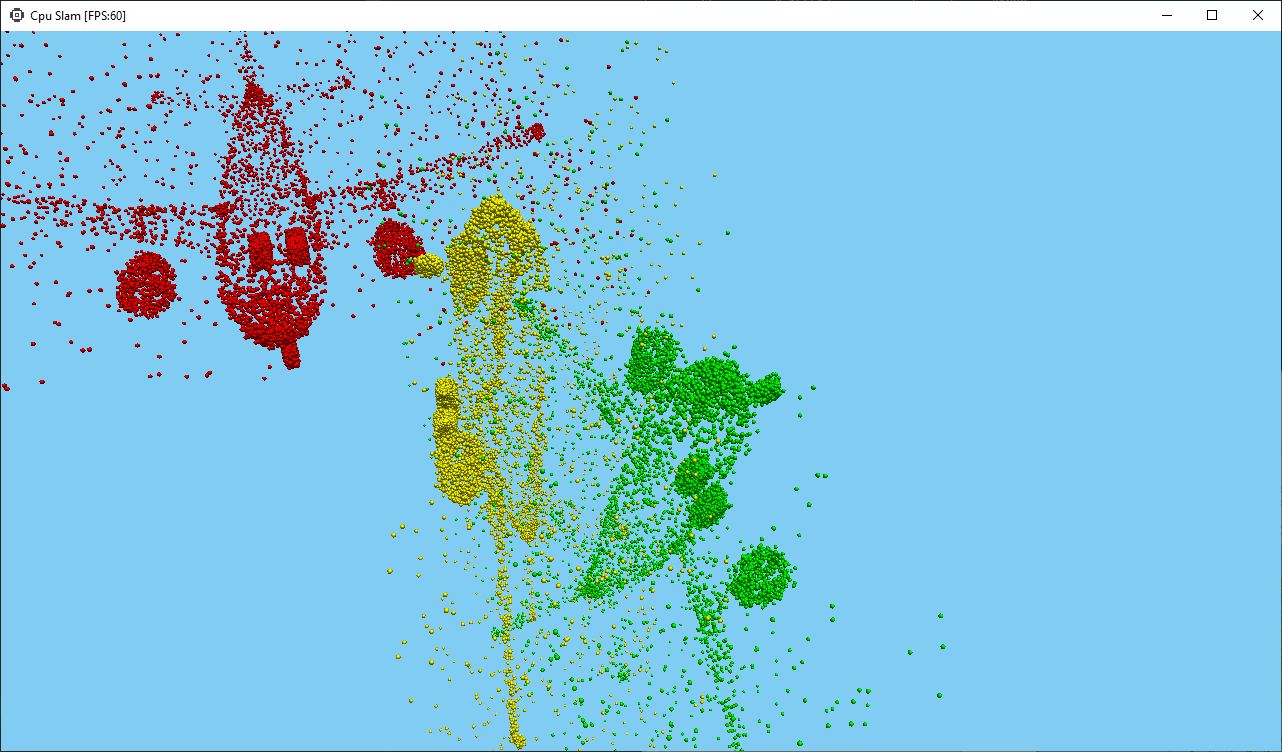
\includegraphics[width=5cm]{mr-icp-21.png} }}
    \hspace{0.5em}
    \subfloat[\centering NICP]{{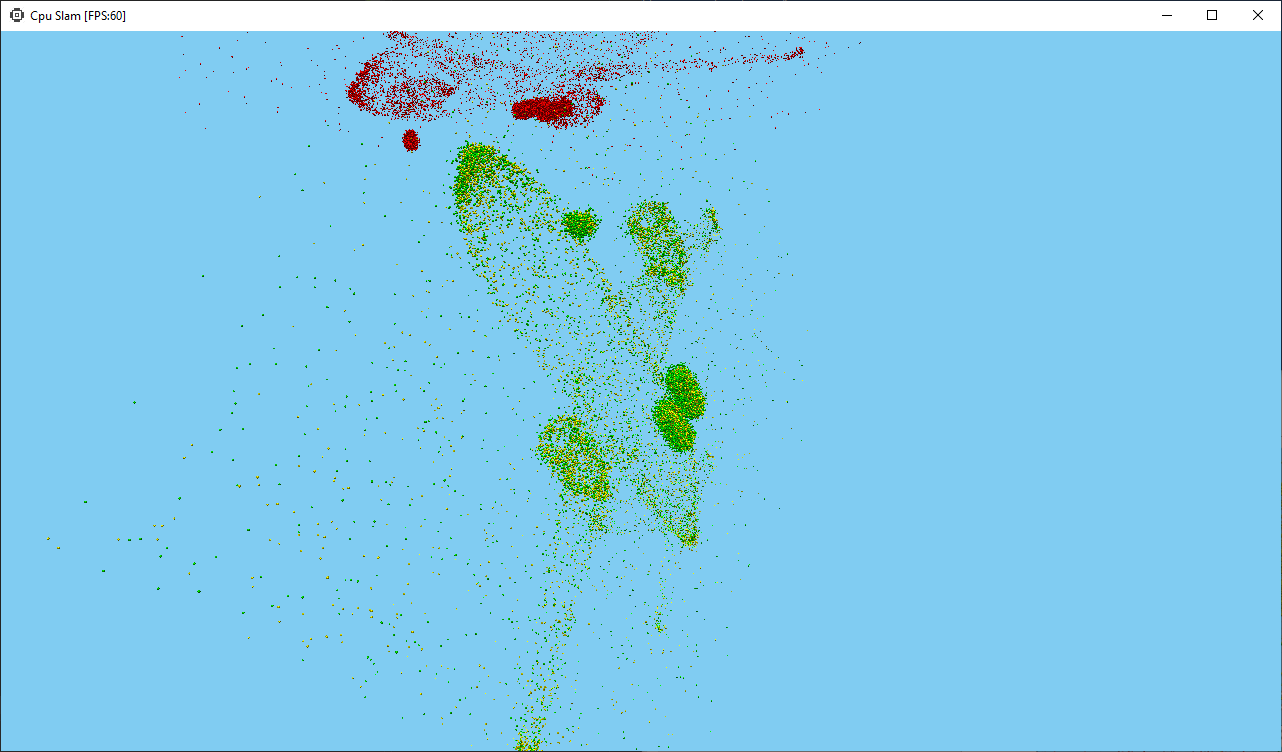
\includegraphics[width=5cm]{mr-nicp-21.png} }}
    \caption{Tests with \textit{Config21.json}}
\end{figure}

The ICP did not manage to converge in this example but result achieved by CPD is interesting. Algorithm connected wheels and engines of both airplanes. Feasibly that is because those are areas with highest point density in entire cloud. NICP returned exact transformation.

Similar situation was met using \textit{Config11.json} and \textit{Config18.json}. Unfortunately in tests using the latter ICP returned identity matrix. The results are presented below.

\begin{figure}[H]
	\centering
    \subfloat[\centering CPD]{{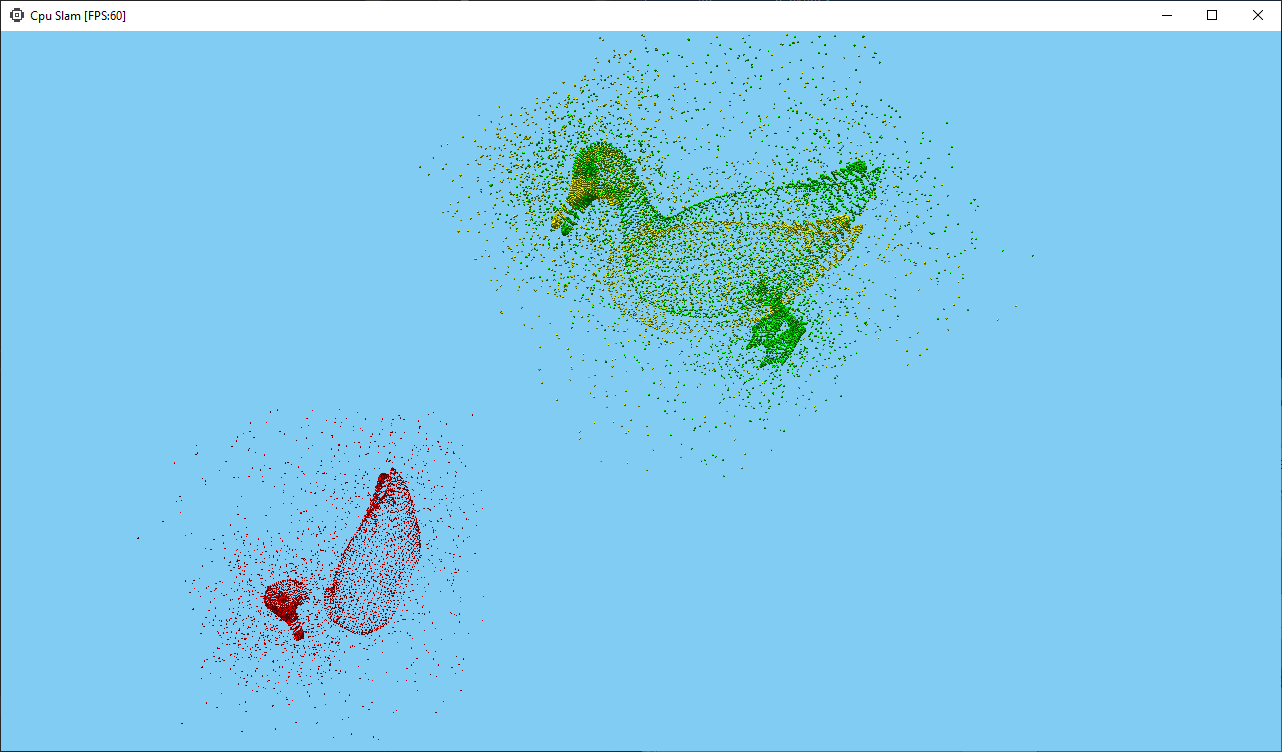
\includegraphics[width=5cm]{mr-cpd-11.png} }}
    \hspace{0.5em}
    \subfloat[\centering ICP]{{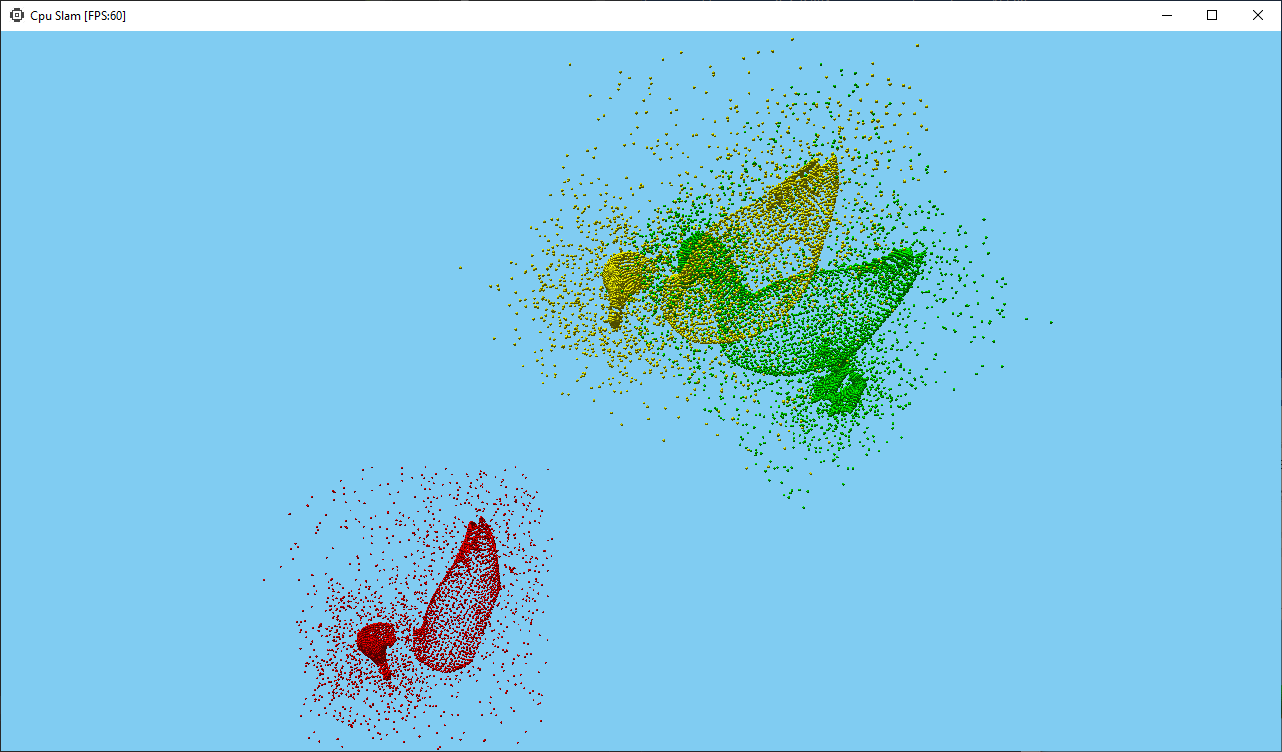
\includegraphics[width=5cm]{mr-icp-11.png} }}
    \hspace{0.5em}
    \subfloat[\centering NICP]{{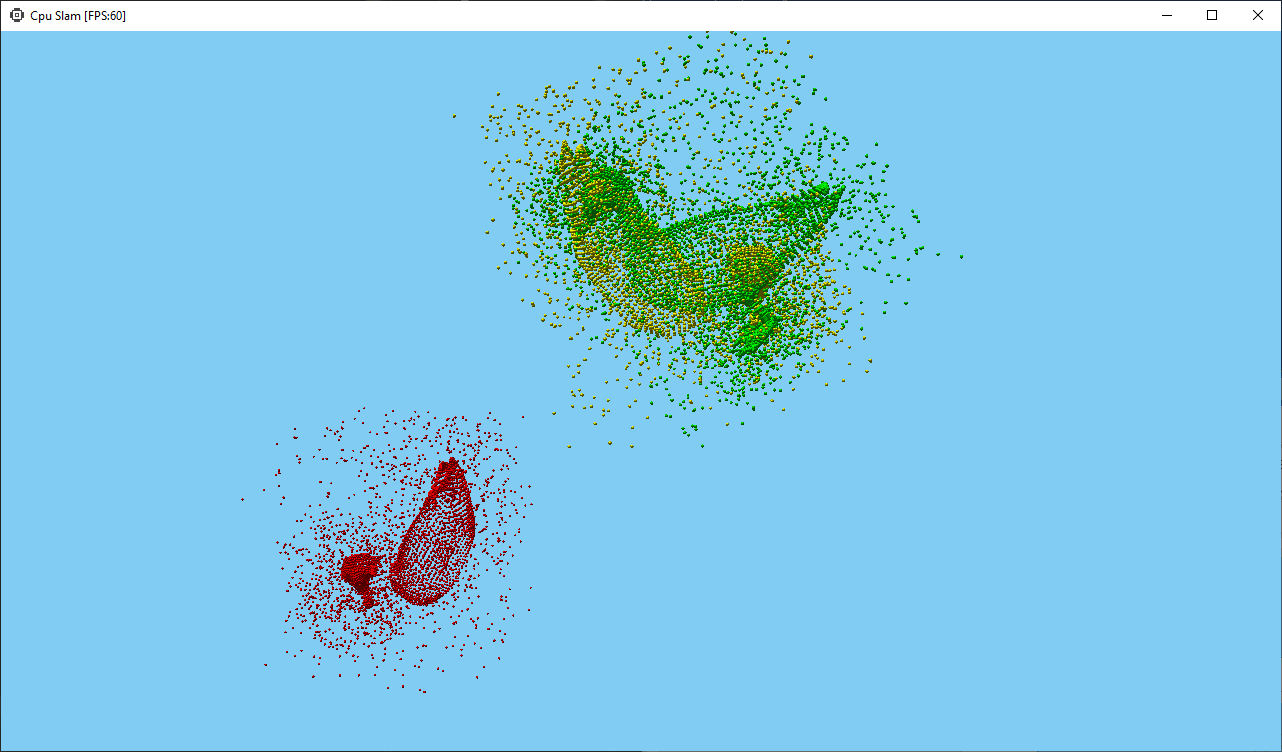
\includegraphics[width=5cm]{mr-nicp-11.png} }}
    \caption{Tests with \textit{Config11.json}}
\end{figure}

\begin{figure}[H]
	\centering
    \subfloat[\centering CPD]{{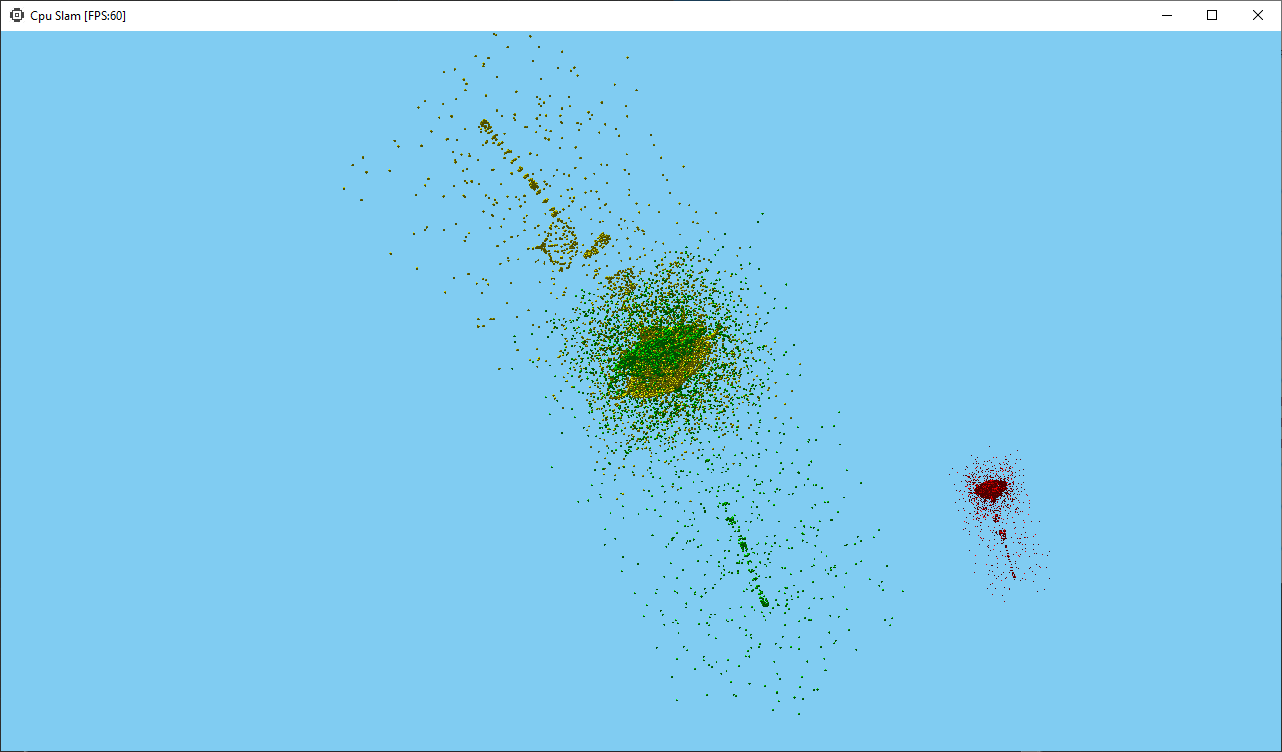
\includegraphics[width=6cm]{mr-cpd-18.png} }}
    \hspace{0.5em}
    \subfloat[\centering NICP]{{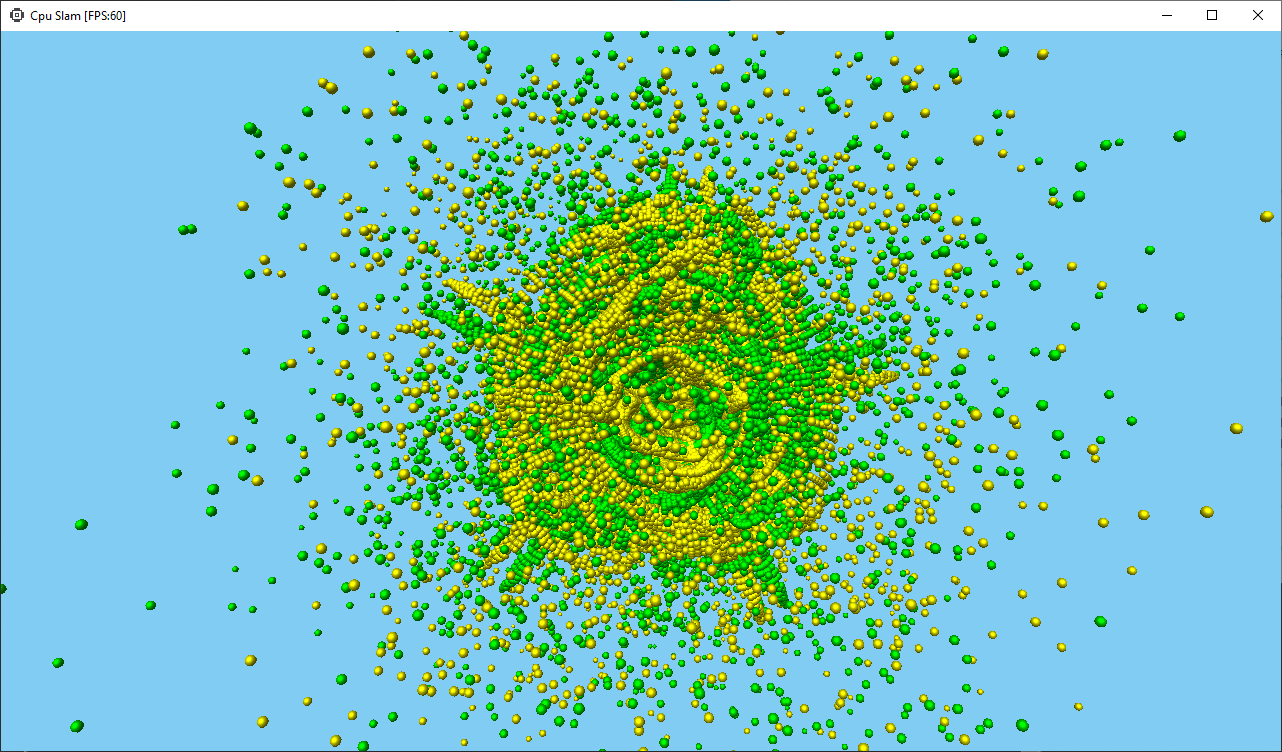
\includegraphics[width=6cm]{mr-nicp-18.png} }}
    \caption{Tests with \textit{Config18.json}}
\end{figure}

In contrary to \textit{Config18.json} and \textit{Config21.json}, using \textit{Config11.json} CPD almost found exact solution while this time NICP focused on matching areas with highest density.

Another example of CPD accuracy in tough conditions can be found when using \textit{Config26.json}. We used two "airbus" clouds where first had no wheels, engines and vertical stabilizer. The second one had wings and wheels cut. Also we have added noise and outliers to both clouds. Results are presented below.

\begin{figure}[H]
	\centering
    \subfloat[\centering CPD]{{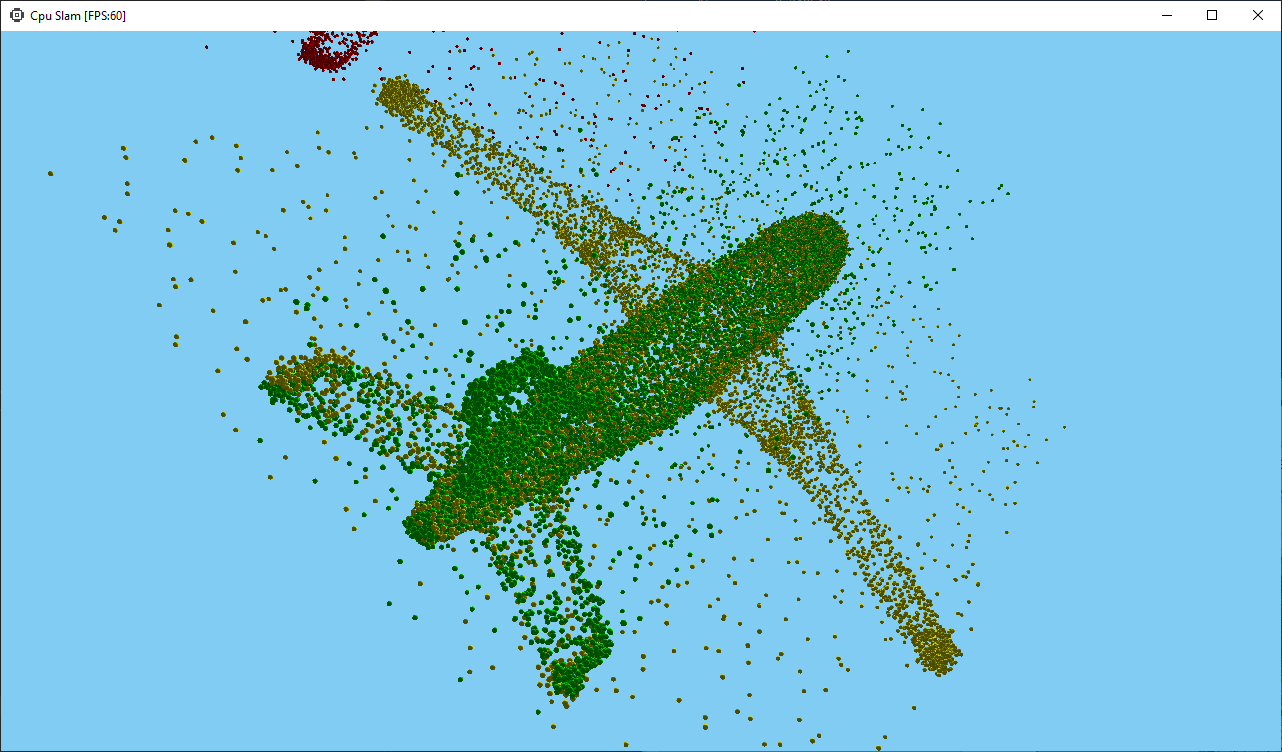
\includegraphics[width=5cm]{mr-cpd-26.png} }}
    \hspace{0.5em}
    \subfloat[\centering ICP]{{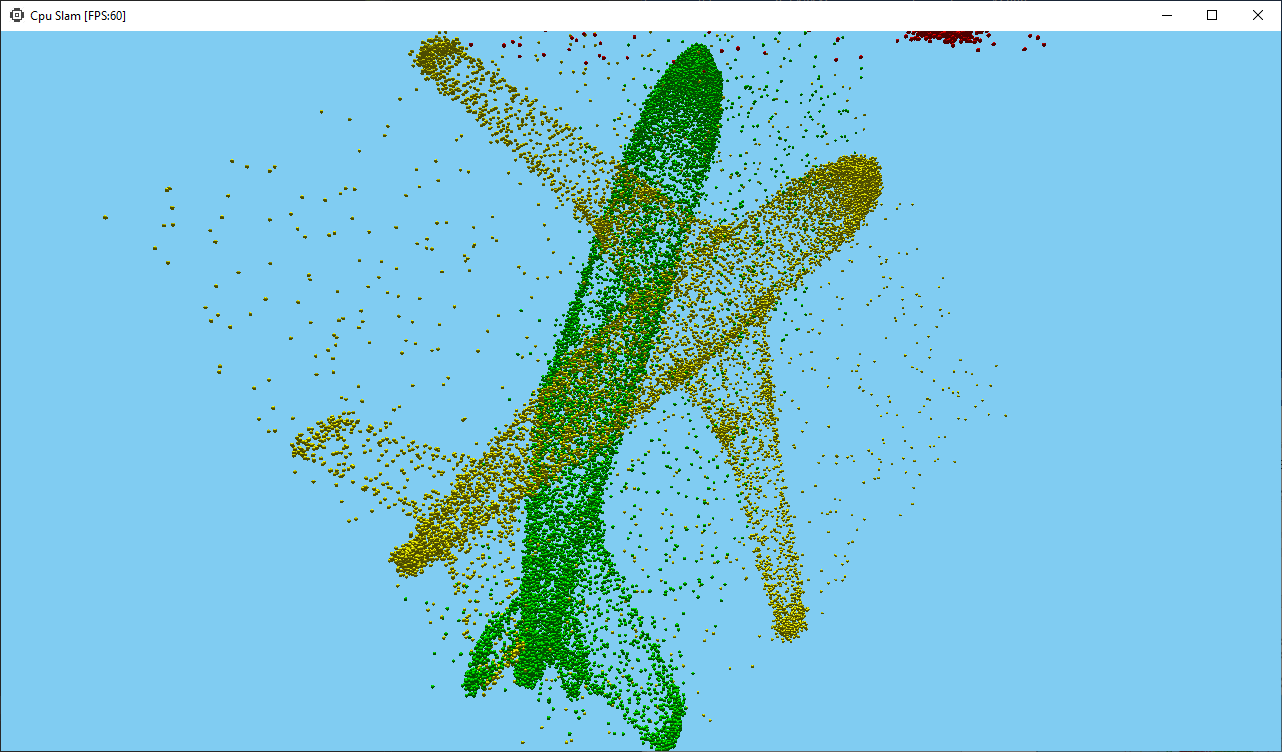
\includegraphics[width=5cm]{mr-icp-26.png} }}
    \hspace{0.5em}
    \subfloat[\centering NICP]{{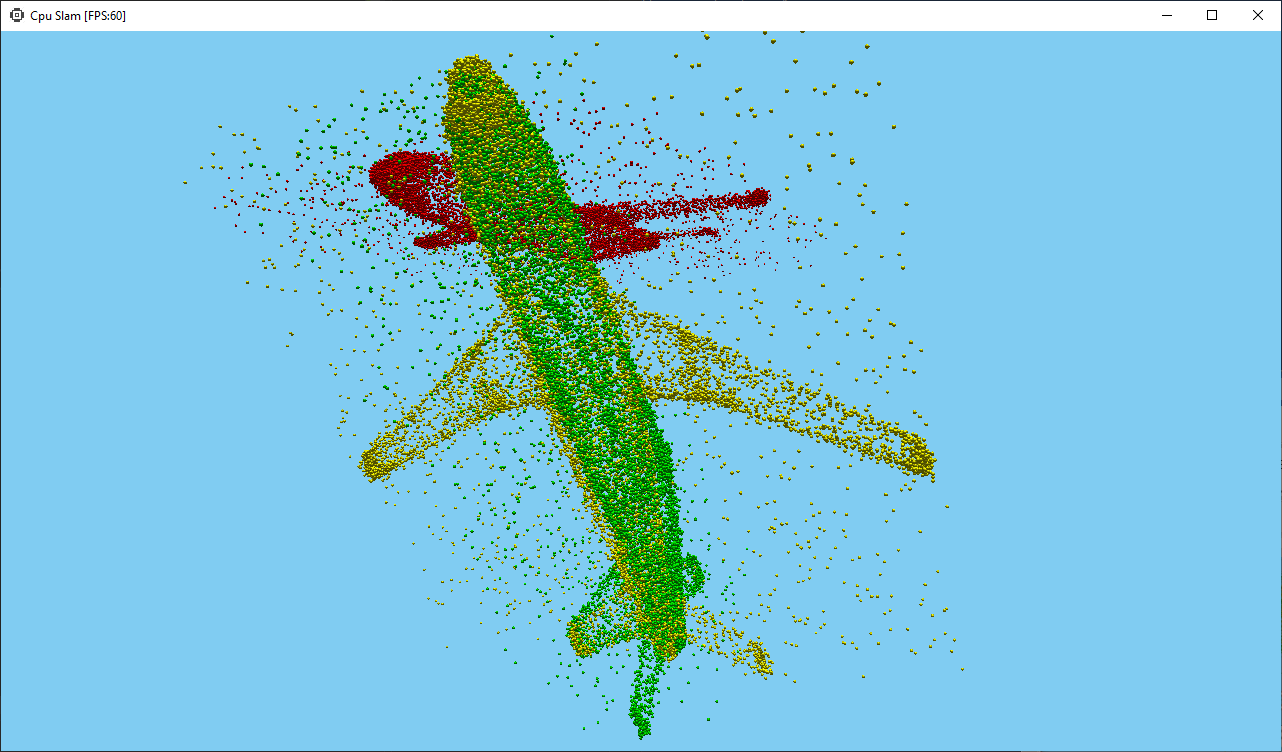
\includegraphics[width=5cm]{mr-nicp-26.png} }}
    \caption{Tests with \textit{Config26.json}}
\end{figure}

CPD found exact solution. As mentioned above ICP has trouble with incomplete clouds and it remains unchanged with this configuration. NICP was close to finding exact solution; however, it lacks of $90\degree$ rotation.

Finally we made test that only focus on situation where one cloud contains noise. We increased the \textit{noise-intensity} by small values and compared the results. The best method occurred to be NICP, CPD was the second and ICP was the third one. For tests, the configurations \textit{Config28.json} to \textit{Config38} were used. Results are presented below.

\begin{figure}[H]
	\centering
    \subfloat[\centering CPD]{{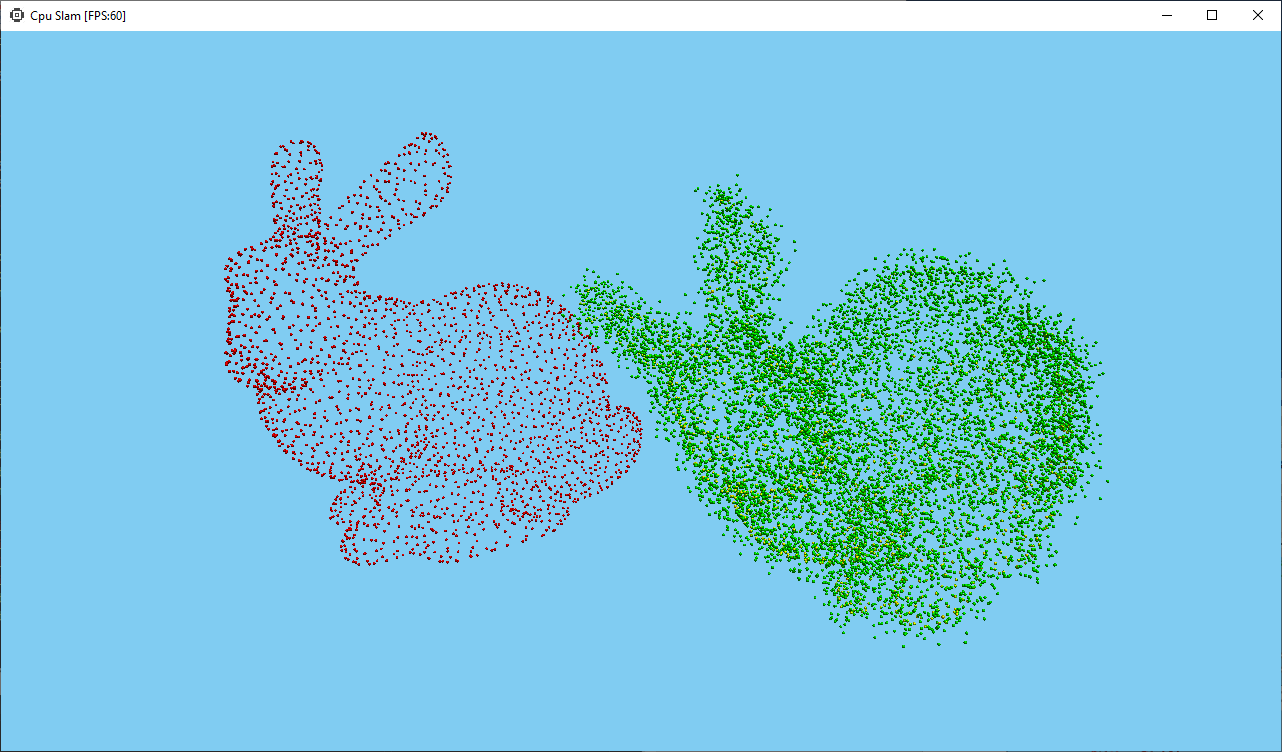
\includegraphics[width=5cm]{mr-cpd-29.png} }}
    \hspace{0.5em}
    \subfloat[\centering ICP]{{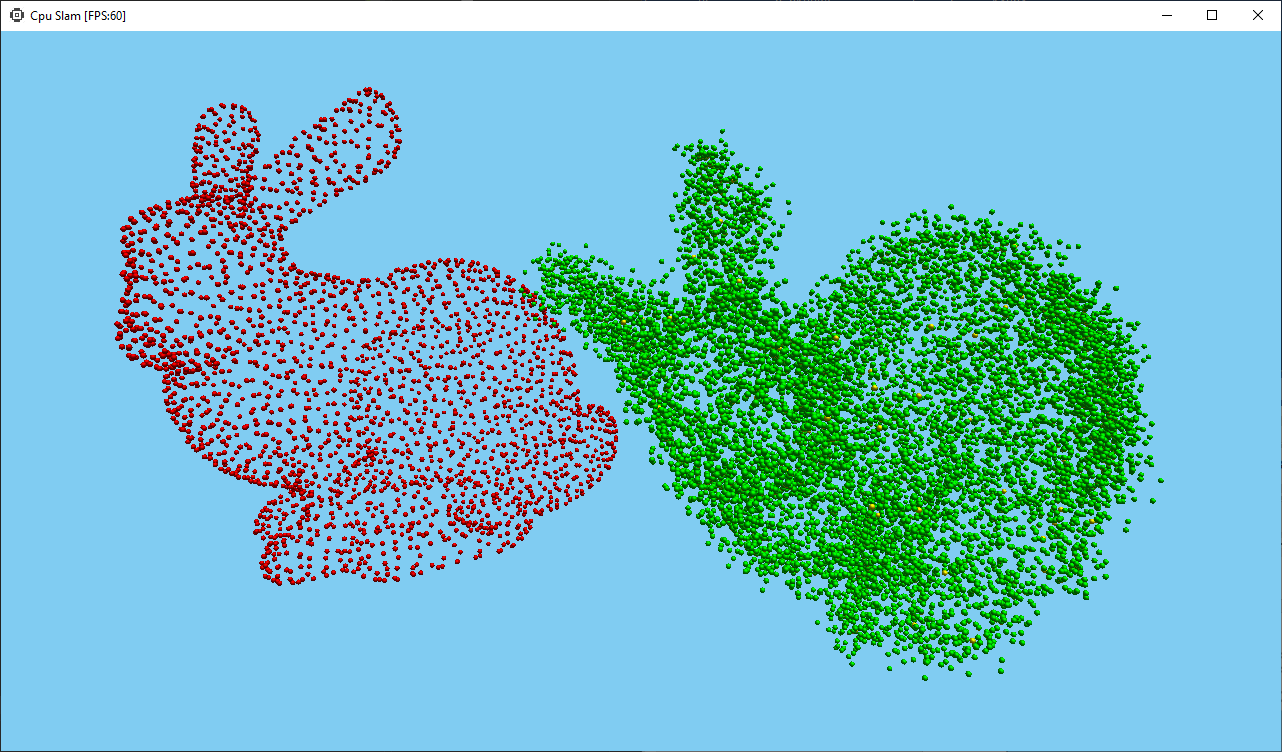
\includegraphics[width=5cm]{mr-icp-29.png} }}
    \hspace{0.5em}
    \subfloat[\centering NICP]{{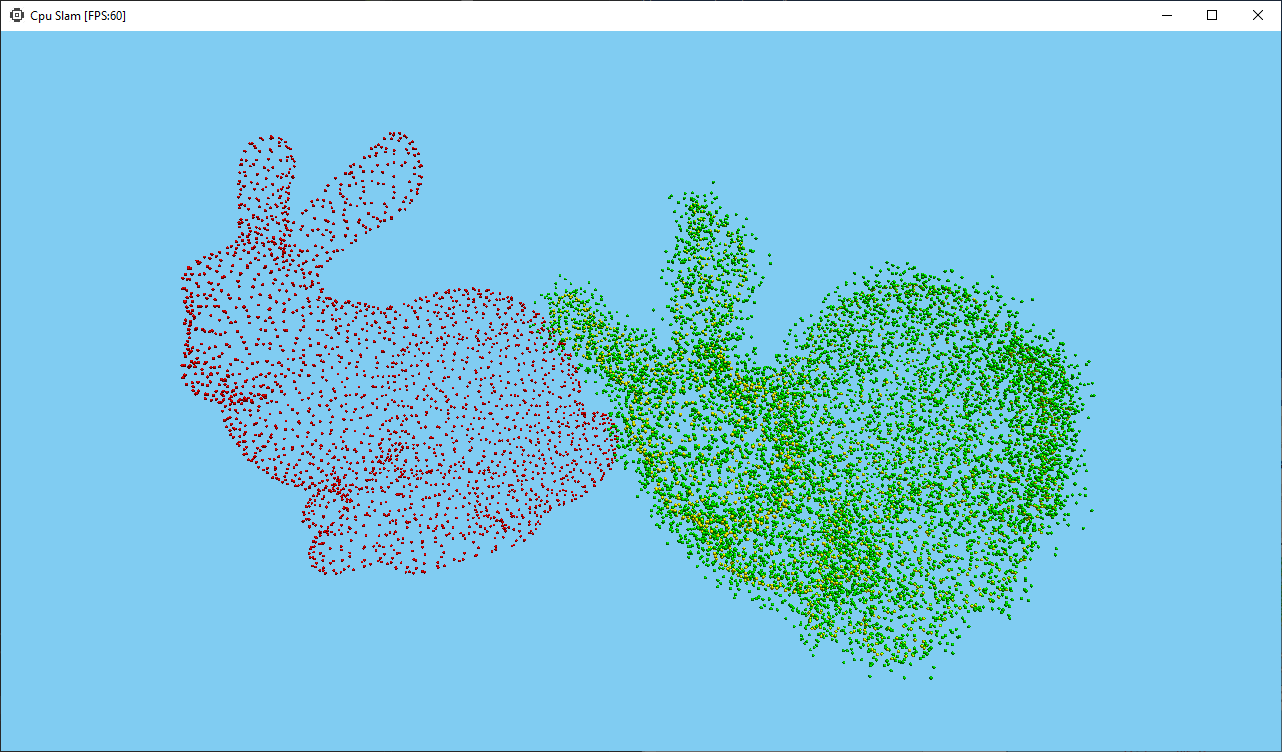
\includegraphics[width=5cm]{mr-nicp-29.png} }}
    \caption{Tests with \textit{Config29.json}}
\end{figure}

\begin{figure}[H]
	\centering
    \subfloat[\centering CPD]{{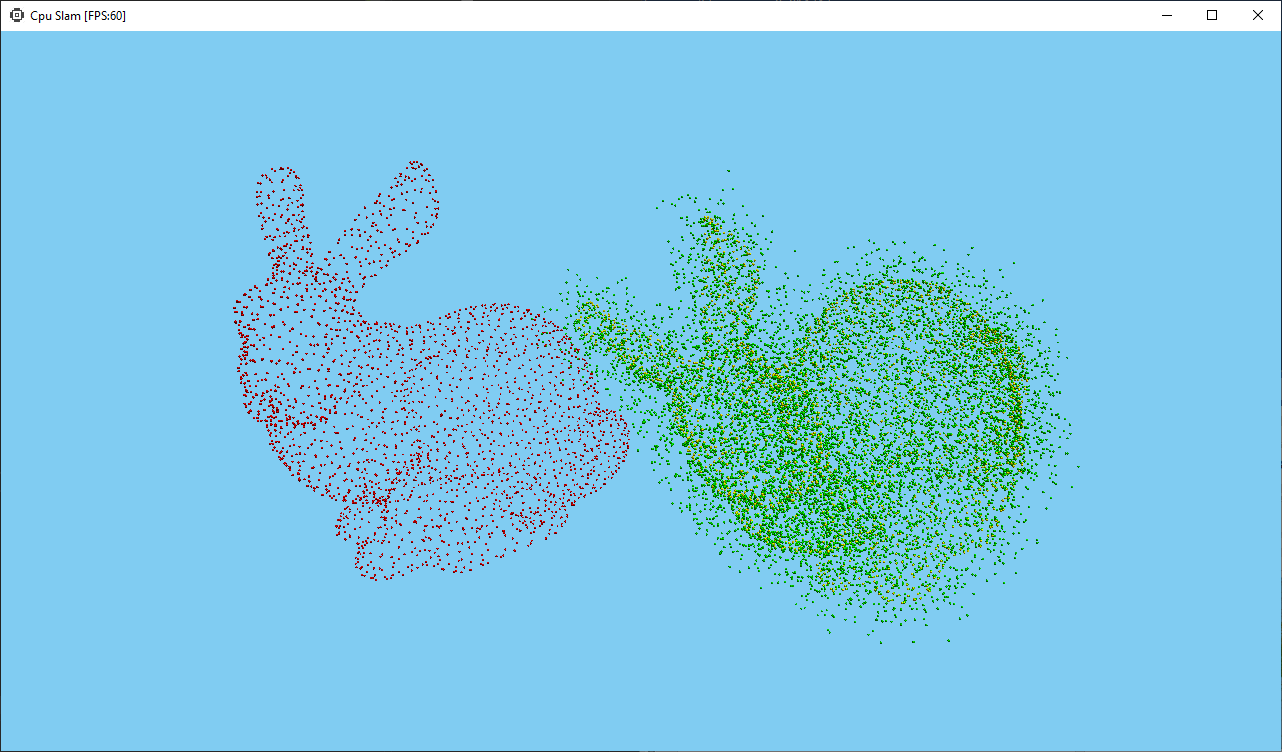
\includegraphics[width=5cm]{mr-cpd-30.png} }}
    \hspace{0.5em}
    \subfloat[\centering ICP]{{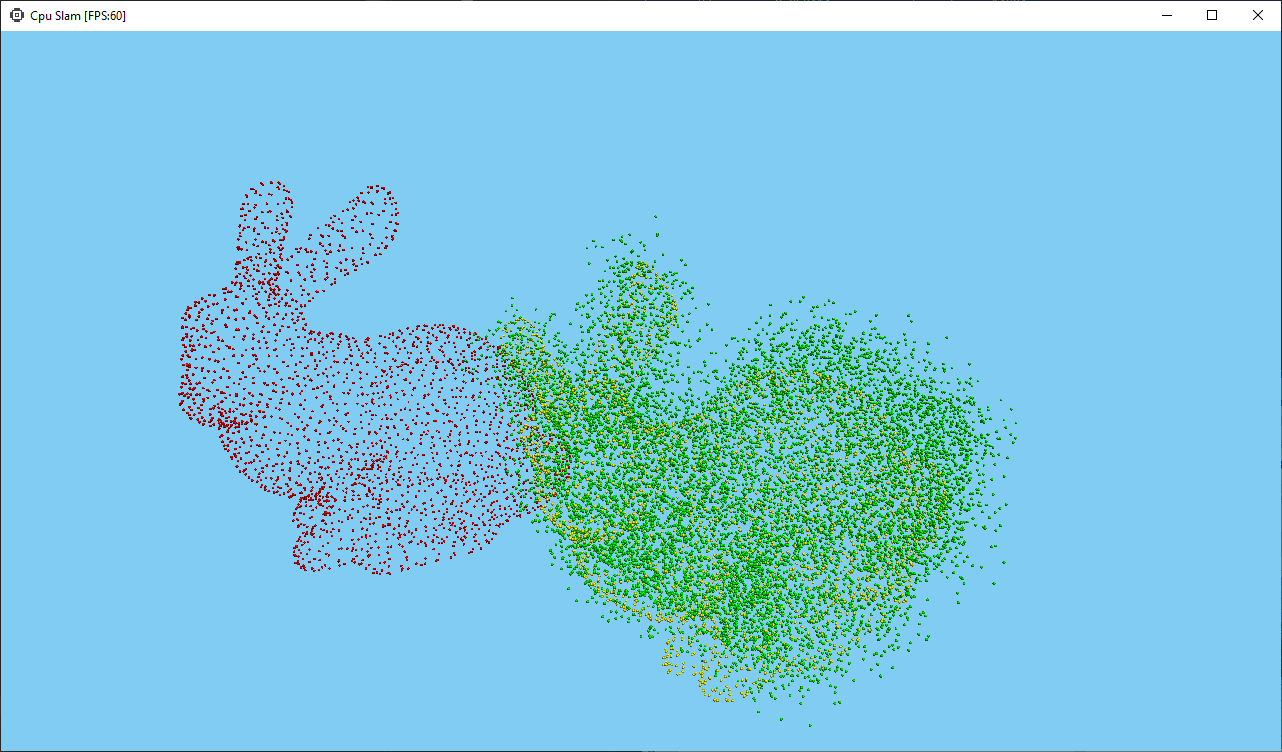
\includegraphics[width=5cm]{mr-icp-30.png} }}
    \hspace{0.5em}
    \subfloat[\centering NICP]{{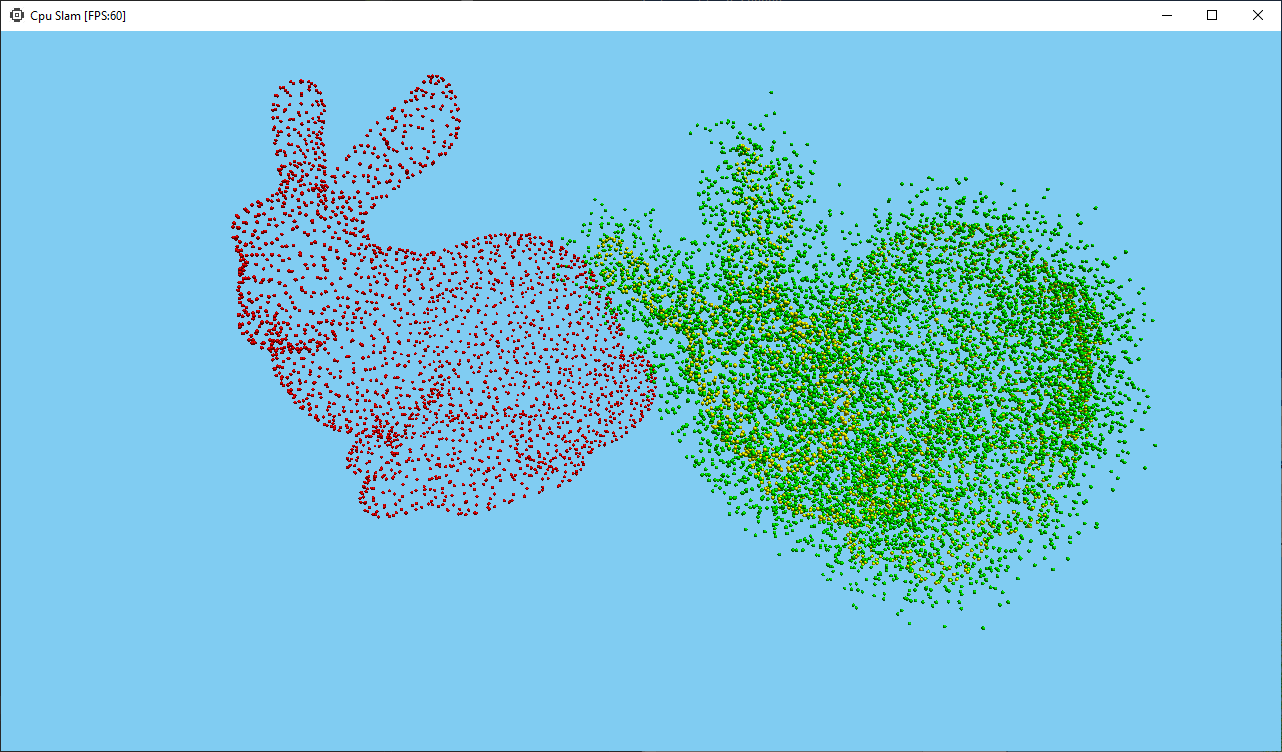
\includegraphics[width=5cm]{mr-nicp-30.png} }}
    \caption{Tests with \textit{Config30.json}}
\end{figure}

\begin{figure}[H]
	\centering
    \subfloat[\centering CPD]{{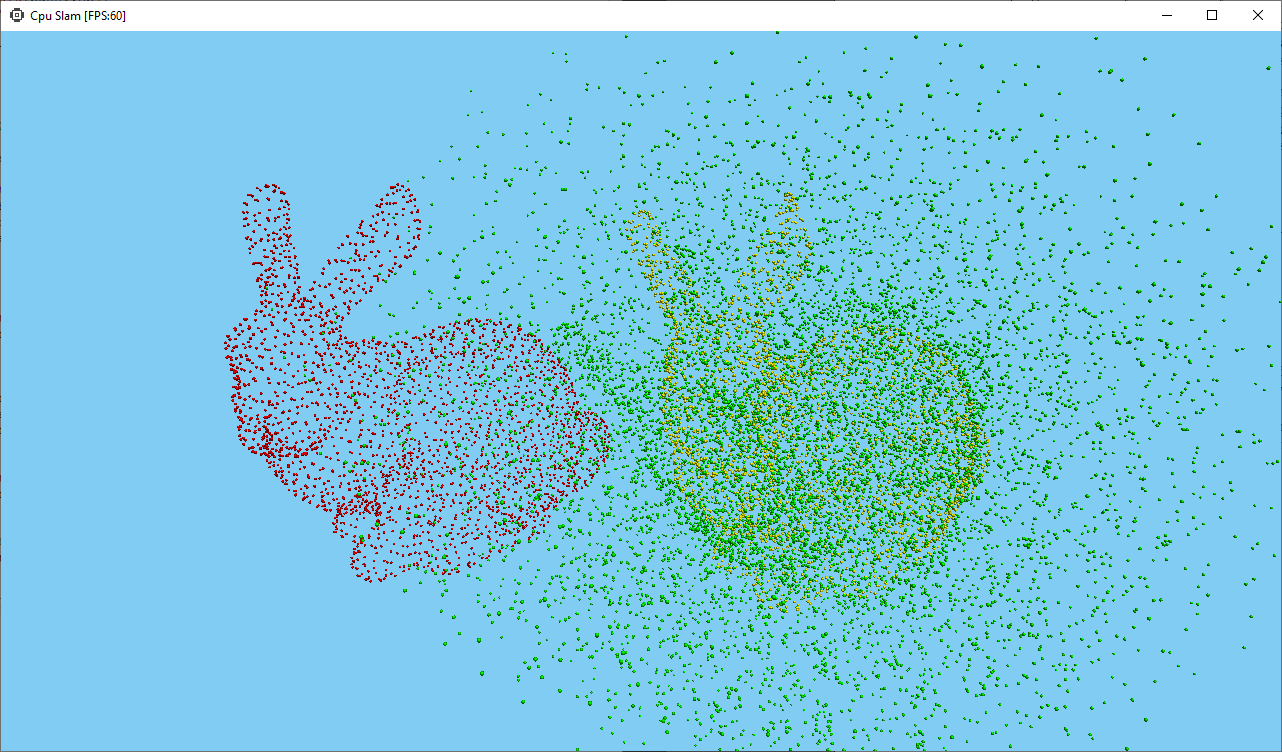
\includegraphics[width=5cm]{mr-cpd-34.png} }}
    \hspace{0.5em}
    \subfloat[\centering ICP]{{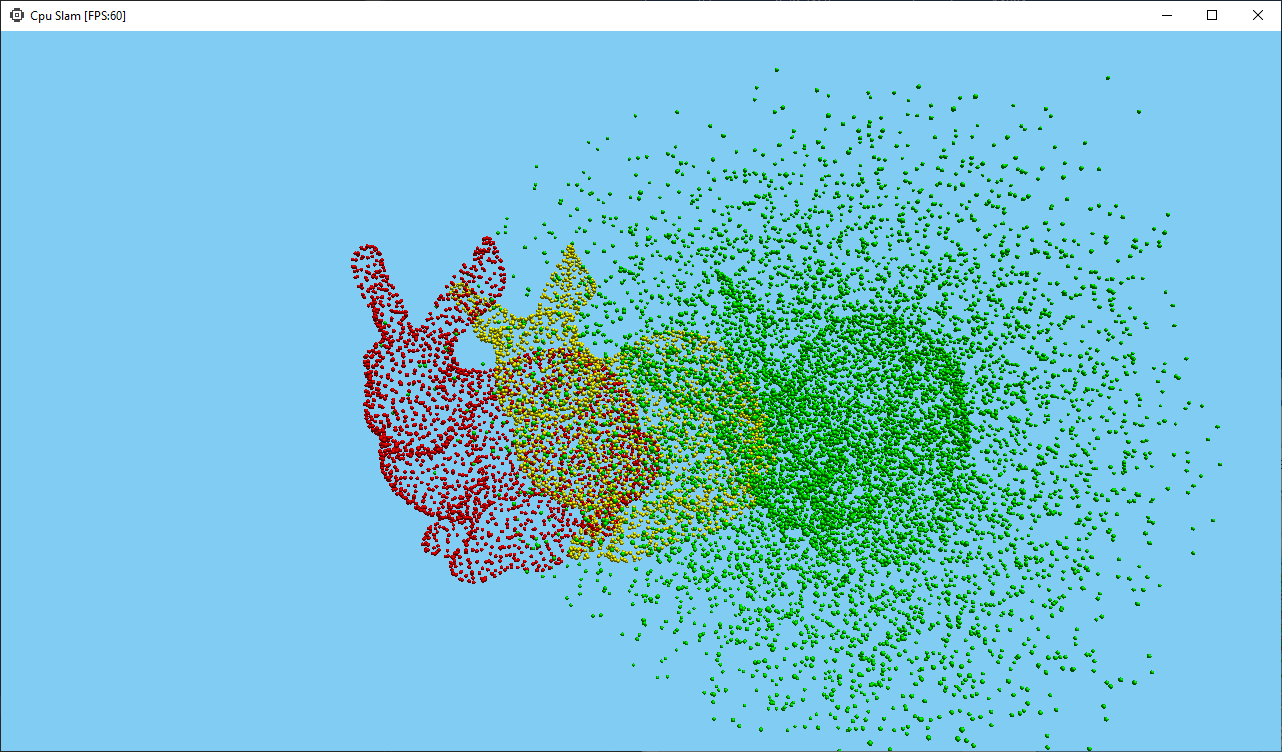
\includegraphics[width=5cm]{mr-icp-34.png} }}
    \hspace{0.5em}
    \subfloat[\centering NICP]{{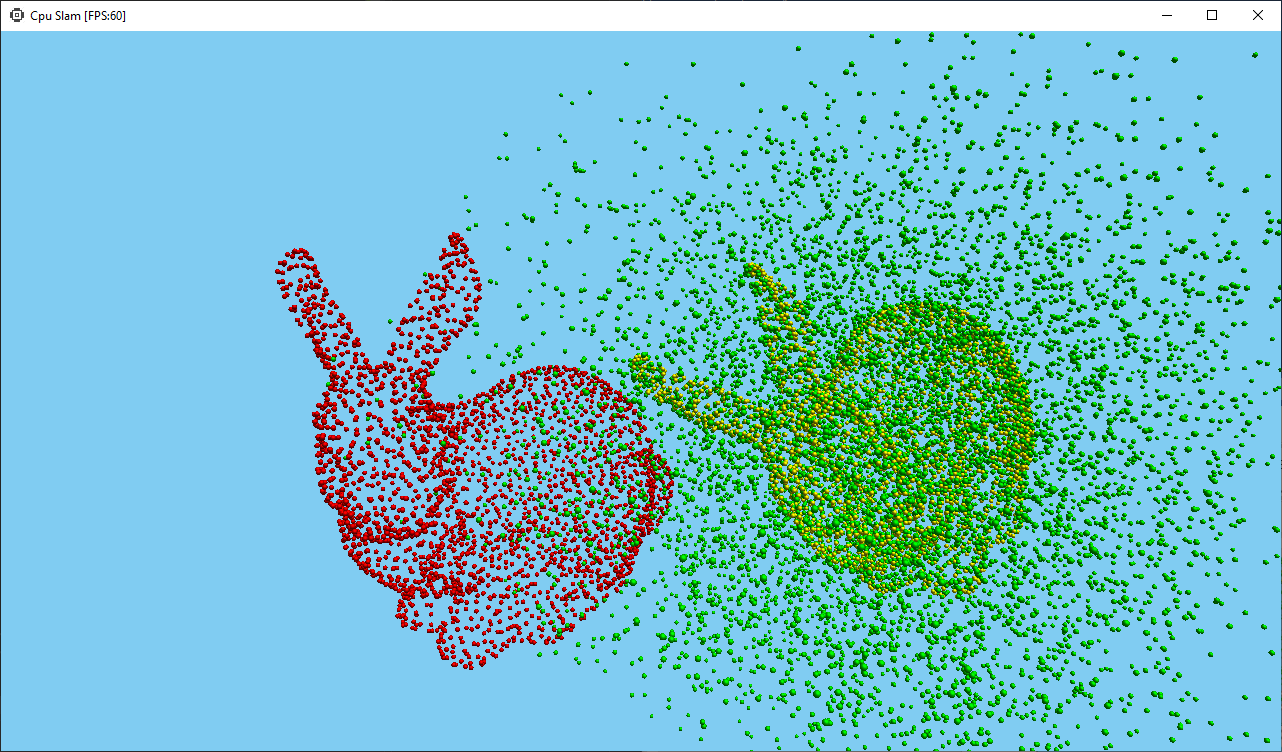
\includegraphics[width=5cm]{mr-nicp-34.png} }}
    \caption{Tests with \textit{Config34.json}}
\end{figure}

\begin{figure}[H]
	\centering
    \subfloat[\centering CPD]{{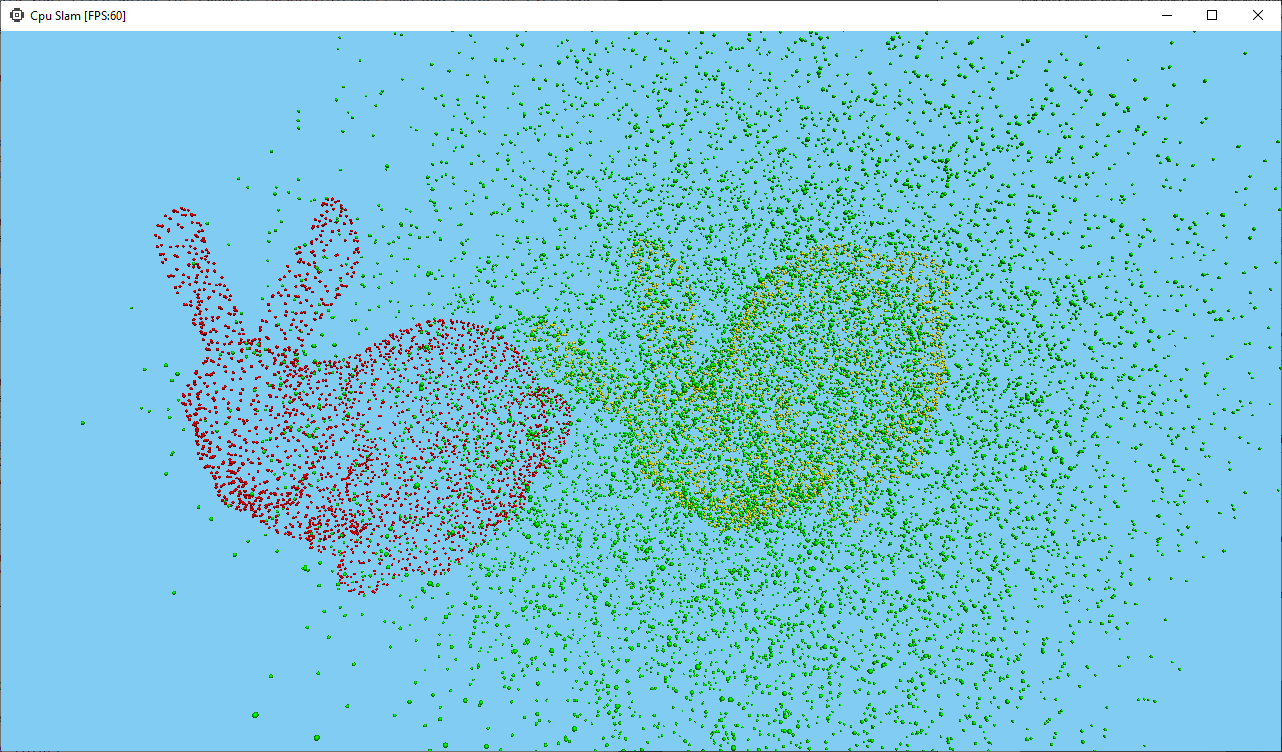
\includegraphics[width=5cm]{mr-cpd-38.png} }}
    \hspace{0.5em}
    \subfloat[\centering ICP]{{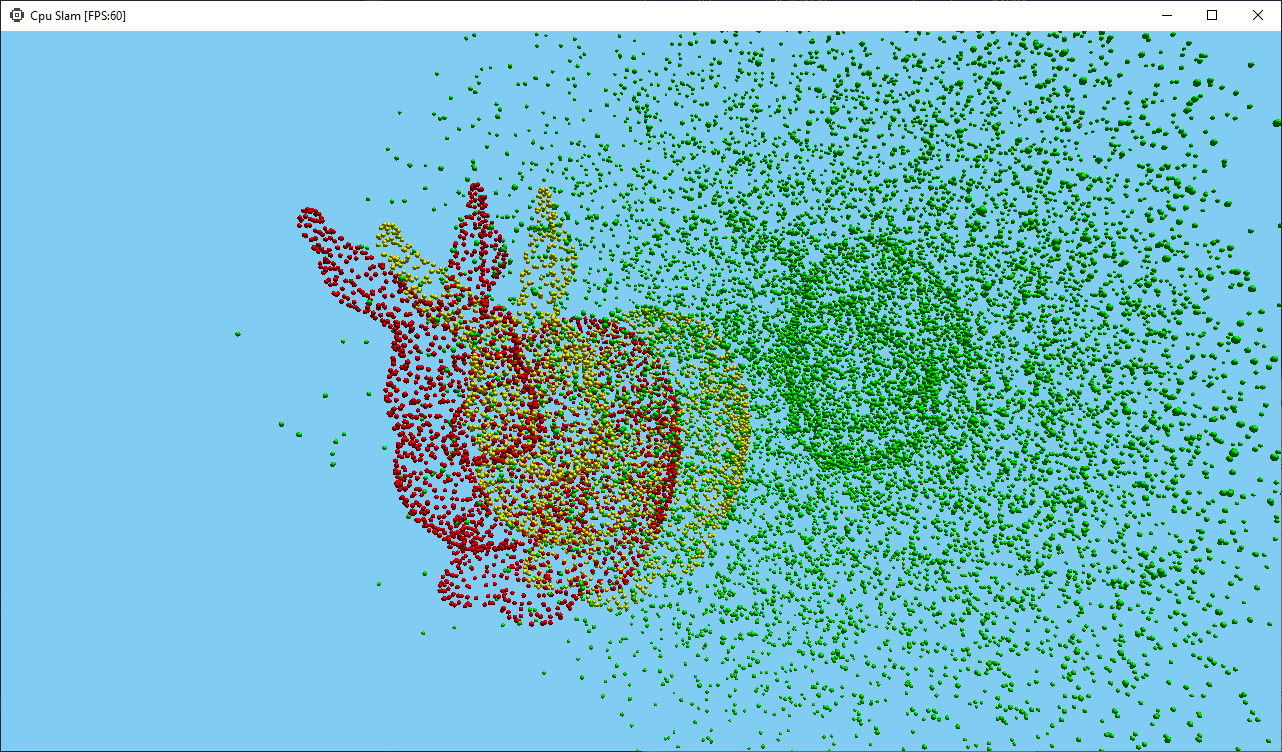
\includegraphics[width=5cm]{mr-icp-38.png} }}
    \hspace{0.5em}
    \subfloat[\centering NICP]{{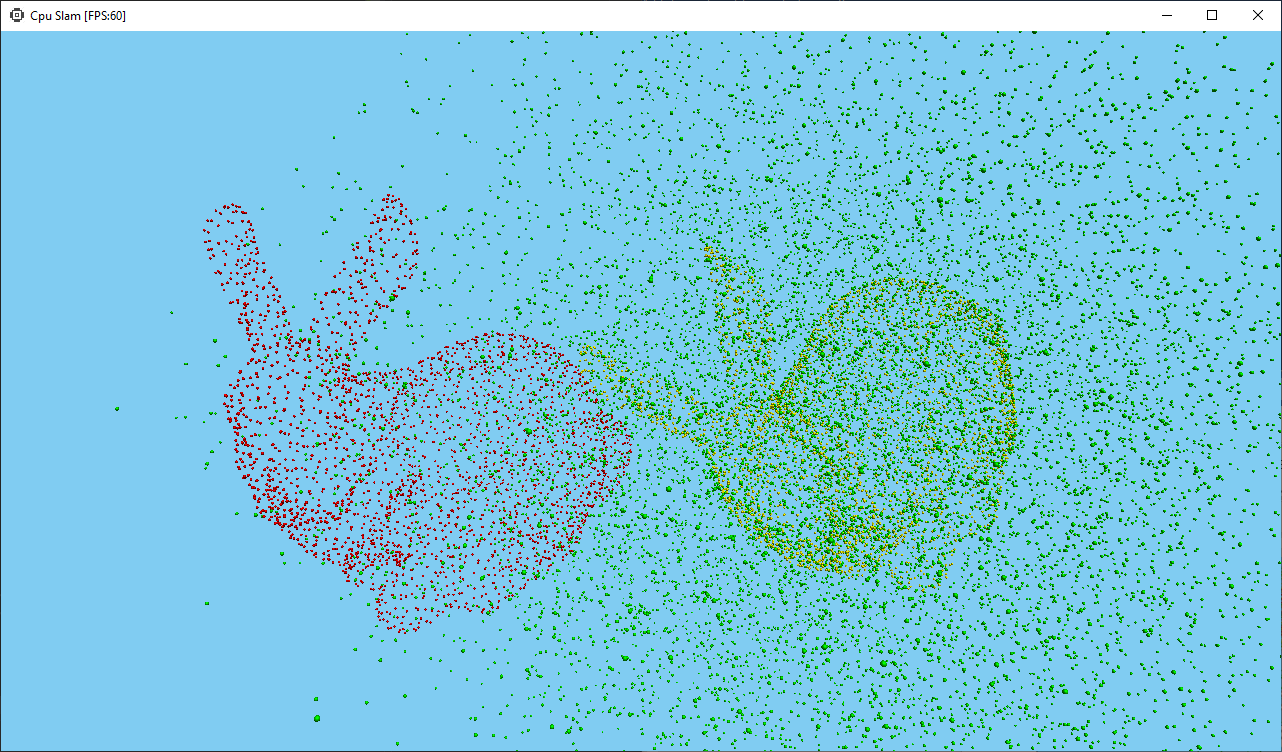
\includegraphics[width=5cm]{mr-nicp-38.png} }}
    \caption{Tests with \textit{Config38.json}}
\end{figure}

NICP managed to find exact solution in all test cases. Results obtained by CPD were slightly worse and sometimes correction of \textit{cpd-weight} parameter was needed. ICP results started to differ even when \textit{noise-intensity} was still very small, thus its usage when conditions are not perfect is very limited.

To sum up the best algorithms for clouds with noises and outliers are NICP and CPD. It is worth mentioning that NICP is significantly faster than CPD. 


\subsection{Convergence ranges}

\subsubsection{Introduction}
Another topic for discussion when it comes to methods' usability is a quality of their results. This section covers convergence rates for all the algorithms, depending on cloud sizes, rotation and translation. Another parameters are same for all the tests, including cloud spread equal to $10$. For all the methods, both GPU and CPU implementations, tests have covered three different translation ranges: 10, 20 and 30 units and three different rotation ranges: 0.2, 0.4 and 0.6 radians, which are equal to 11.5\degree, 22.9\degree and 34.4\degree respectively.

Based on the performance results from previous sections, cloud sizes have been chosen separately for each method and they differ significantly from each other, but remain the same between GPU and CPU implementation of a specific method. It is also worth noting that for methods with multiple approximation types, only one type is chosen for tests and the decision is described in the section focusing on specific method.

\subsubsection{Iterative closest point}
In case of an ICP, convergence rates are deeply correlated with a maximum number of iterations the algorithm runs. And this turns out to be the main drawback of this method. In order to compare methods most fairly, we had to limit the iterations in a way that keeps computation times close to the other methods. At the same time, we needed to keep similar parameters for both CPU and GPU implementation and for this reason iterations have been limited by $100$. Cloud sizes have been chosen from range $[20000,100000]$ which positions ICP in the middle of the road between CPD and Non-iterative Closest Point.

Unfortunately, it is noticeable from the chart below that for large clouds, convergence rate falls dramatically. It is caused mainly by limiting the iterations mentioned above. In most of the test cases, the error in consecutive iterations tended to fall down, but the dynamics of changes did not allow the algorithm to converge in acceptable time.
\begin{figure}[H]
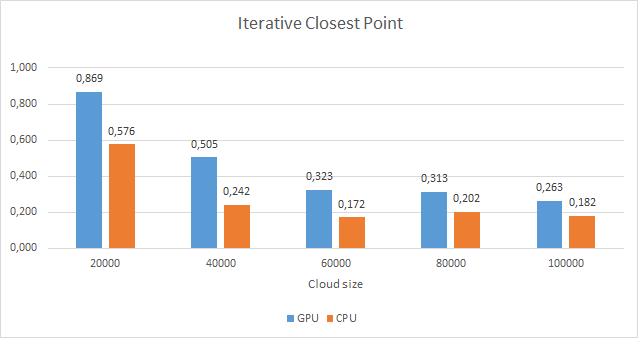
\includegraphics[width=\textwidth]{ss-icp-1.png}
\caption{Convergance rates for ICP depending on cloud size}
\end{figure}
The situation is slightly different when it comes to comparing ICP efficiency based on translation between first and second point cloud. In this case, the differences are not so grand and only large translation cause the visible decrease of convergence rate. What is worth mentioning are the differences between GPU and CPU implementation. GPU turns out to be even more than 5 times better when it comes to matching clouds with large translation. This may indicate lower accuracy of math libraries used on CPU, especially for decomposition of matrices with larger values. 
\begin{figure}[H]
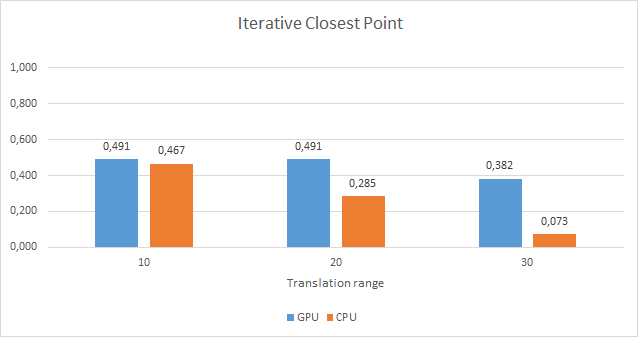
\includegraphics[width=\textwidth]{ss-icp-2.png}
\caption{Convergance rates for ICP depending on translation}
\end{figure}
The differences between GPU and CPU computations are not that evident if we compare the rotated clouds. In this situation, the CPU implementation tend to maintain similar convergence rate, despite the rotation value. The overall GPU dynamics in this case is the same as for the tests based on translation.
\begin{figure}[H]
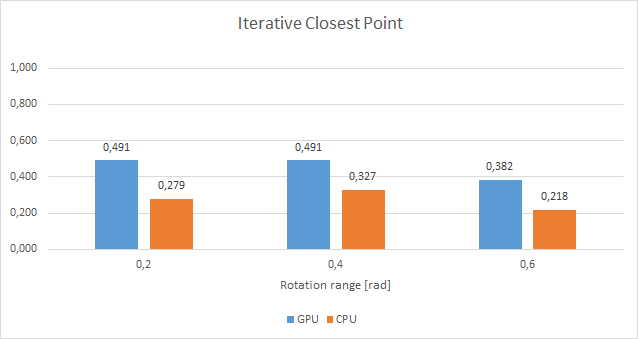
\includegraphics[width=\textwidth]{ss-icp-3.png}
\caption{Convergance rates for ICP depending on rotation}
\end{figure}
Summarizing the convergence tests for an ICP algorithm, the method does not show great differences between convergence rate based on translation and rotation, but the rates are in all the cases rather low. The method's advantage is the possibility of significantly improving the results by increasing the number of allowed iterations. In most of the test cases, it was this limitation, not the maximum error what caused the computations to stop.

\subsubsection{Non-iterative closest point}
Non-iterative closest point method is the first one for which different approximation types have been implemented. However, the execution times proved that only one type is worth using in general cases. For this reason, the "None" type is used in all convergence tests, as it not only gives the most accurate results, but it also offers execution time unsurpassed by other methods.

Performance tests for proposed implementation showed as well that substantial cloud sizes are not an obstacle for a Non-iterative Closest Point algorithm and because of that, the sizes used in the convergence tests vary between 250000 and 1250000. Nevertheless, execution times are still lower than for the other algorithms.

Not only the cloud sizes and execution times are surpassing other methods, but convergence rates show similar tendency. The overall convergence rate for non-iterative method was equal to 1.0 for GPU implementation and 0.99 for CPU. The impact of specific parameters on the results is displayed on charts below.
\begin{figure}[H]
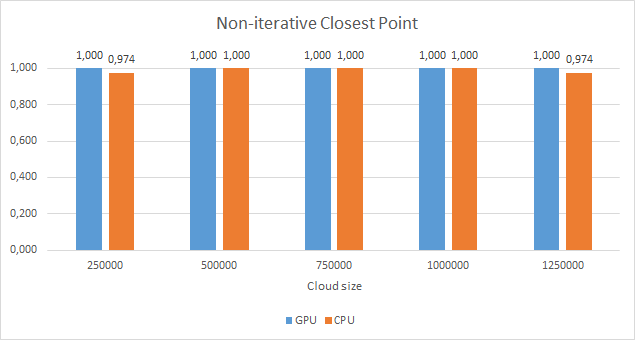
\includegraphics[width=\textwidth]{ss-nicp-1.png}
\caption{Convergance rates for a non-iterative closest point matching depending on cloud size}
\end{figure}
\begin{figure}[H]
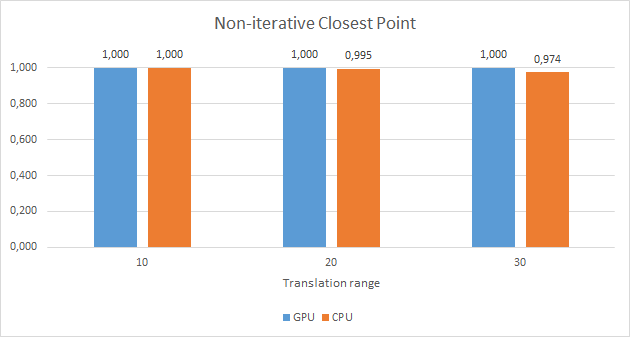
\includegraphics[width=\textwidth]{ss-nicp-2.png}
\caption{Convergance rates for a non-iterative closest point matching depending on translation}
\end{figure}
\begin{figure}[H]
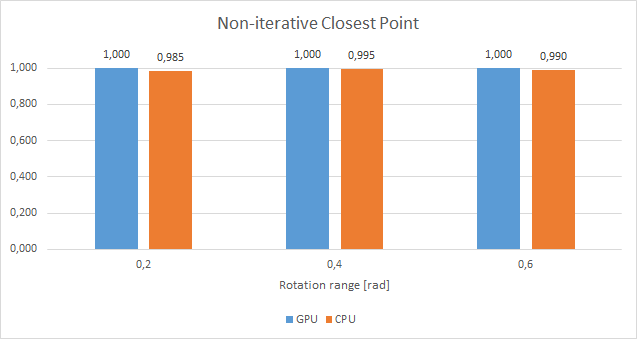
\includegraphics[width=\textwidth]{ss-nicp-3.png}
\caption{Convergance rates for a non-iterative closest point matching depending on rotation}
\end{figure}
The slim disparity between the two variants of implemented method are most likely caused by precision of CPU and GPU matrix operations which strengthens the hypothesis put forward while analysing the ICP algorithm. However, in this case the differences are not so grand which can be caused by reduced number of matrix operation and therefore less error propagation.

\subsubsection{Coherent point drift}
Coherent point drift is another method parametrized by approximation type it uses. In this case, we decided to pick the hybrid variant, guided mainly by performance results and the fact that improvements done by implementing Fast Gauss Transform have no impact on convergence rate. All above make hybrid approximation the most competitive version out of all three implemented.

However, the run times of CPD algorithm are still far lower than for other methods and for that reason cloud sizes chosen are significantly lower being in the range $[4000, 20000]$, still offering the longest computation time. On the other hand, convergence rates are much more competitive comparing to the results of ICP for computations in comparable time.
\begin{figure}[H]
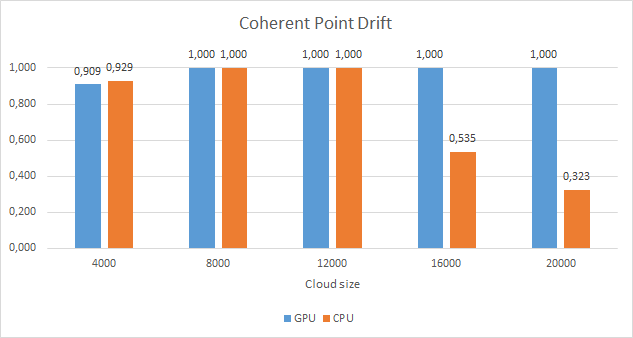
\includegraphics[width=\textwidth]{ss-cpd-1.png}
\caption{Convergence rates for a non-iterative closest point matching depending on cloud size}
\end{figure}
Nevertheless, the convergence rates of CPU algorithm reveal a trend towards a drastic decline for larger clouds. It is noticeable that for objects of size above 16000 points, rate is even lower than 0.5 when the GPU implementation keeps the results perfectly matched.
This seems to be the case also for increasing translation between clouds. This time the differences are not so grand though.
\begin{figure}[H]
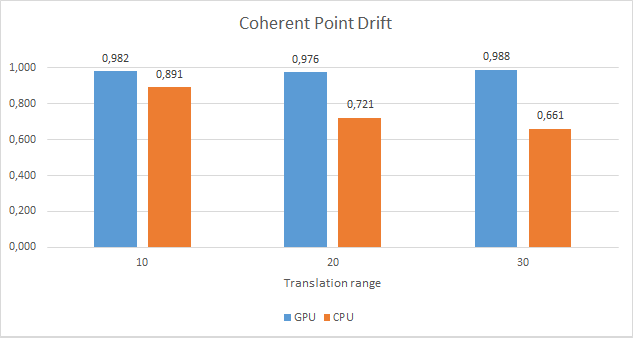
\includegraphics[width=\textwidth]{ss-cpd-2.png}
\caption{Convergence rates for a non-iterative closest point matching depending on translation}
\end{figure}
Modifying rotation of target cloud, the phenomenon described above seems to completely disappear. What is more, larger rotation results in higher convergence rate of tested algorithm but differences between them are significantly lower.
\begin{figure}[H]
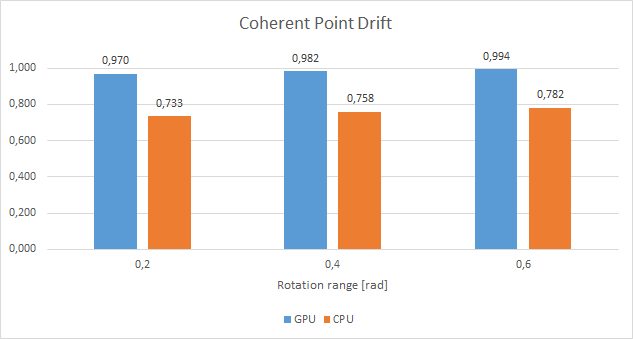
\includegraphics[width=\textwidth]{ss-cpd-3.png}
\caption{Convergence rates for a non-iterative closest point matching depending on rotation}
\end{figure}
Summarizing the convergence of implemented CPD algorithms, we strongly encourage to use GPU version rather than CPU. Even tough computation times can be greater, convergence rate is then kept on similar and very high level above 0.9. This method is also the only one that can match scaled clouds which makes it more universal. 

Once again, CPU implementation gives far worse results than the GPU one. For this method that might be caused by using operations on large matrices not only for SVD but also for a multiplication.

\subsubsection{Methods comparison}
To sum up the convergence tests, the average rate for all tests have been calculated for each method, with division to GPU and CPU implementation. Based on that, it is easier to visualise the results that were already mentioned in all the section. 
\begin{figure}[H]
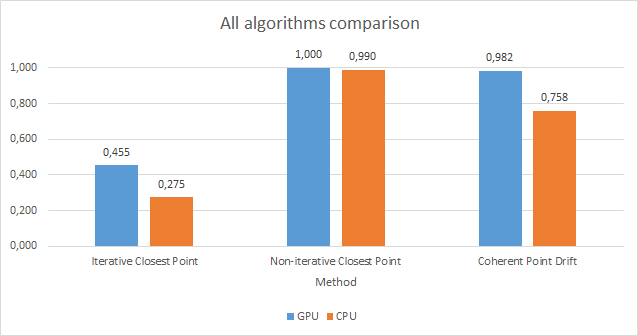
\includegraphics[width=\textwidth]{ss-all.png}
\caption{Comparison of all algorithms convergence rates}
\end{figure}
And once again it is clear that CPD and Non-iterative closest point methods are a lot more accurate when it comes to finding transformation between two point sets.

Another conclusion is that CPU implementation of complicated matrix operations is significantly inferior to the one accelerated by GPU. It might be the case only for the two libraries that were used in this project, however it is worth noting that the CPU library is known for its precision.

\section{Future works}
%What do we want to do in future, improvements.

\subsection{Iterative Closest Point}
We implemented a solid ground base for development of ICP algorithm. There are a lot of ways it can be improved but the most important would be enhancing performance of correspondences step as it is critical for the whole method execution time.

\subsection{Coherent Point Drift}
We implemented whole rigid part of the algorithm on cpu, including FGT. Unfortunately FGT was not implemented on GPU as mentioned in \textit{\ref{sec:ImplementationDetails}. \nameref{sec:ImplementationDetails}}. This is main area of future improvement for GPU solution. Coherent Point Drift also has affine and non-rigid versions that are worth mentioning. There were not implemented because it reaches beyond the scope of our project. Future works can mainly focus on improving GPU solution and moving to non-rigid transformations.

\subsection{Non-iterative Closest Point}
This method is for sure the most narrowly documented among all three described in this report. On the other hand, the idea does not leave much space for improvements. The biggest obstacle to using it on greater scale is undetermined convergence ratio. Although the tests conducted showed that running the algorithm for 20 pseudo-random permutations gives convergence ratio of 100\%, but the actual correlation between computation precision and cloud properties such as size or density remains unknown.\\
Other place for improvements is related closely to implementation issue. Different libraries and methods of computing SVD offers different accuracy. This can be seen for example by comparing results of CPU computations using Eigen library (recommended as one of the top when it comes to finding matrix decomposition) and GPU's cuSOLVER, where for the second one, error is smaller in majority of test cases. There are also multiple other, both closed and open source implementations for both CPU and GPU which might offer better results when it comes to convergence or computation time, especially for some specific cases.

\subsection{Common improvements}
The key to performant SLAM for big clouds is sampling. We have not covered it in our work as it is a broad topic and mostly dependent of the specific application of the algorithm. Although, there is no contraindication to use sampled clouds as the input of our program so everybody can make their own experiments in that field.

\newpage
\printbibliography

\end{document}

